\documentclass[twoside]{book}

% Packages required by doxygen
\usepackage{fixltx2e}
\usepackage{calc}
\usepackage{doxygen}
\usepackage[export]{adjustbox} % also loads graphicx
\usepackage{graphicx}
\usepackage[utf8]{inputenc}
\usepackage{makeidx}
\usepackage{multicol}
\usepackage{multirow}
\PassOptionsToPackage{warn}{textcomp}
\usepackage{textcomp}
\usepackage[nointegrals]{wasysym}
\usepackage[table]{xcolor}

% Font selection
\usepackage[T1]{fontenc}
\usepackage[scaled=.90]{helvet}
\usepackage{courier}
\usepackage{amssymb}
\usepackage{sectsty}
\renewcommand{\familydefault}{\sfdefault}
\allsectionsfont{%
  \fontseries{bc}\selectfont%
  \color{darkgray}%
}
\renewcommand{\DoxyLabelFont}{%
  \fontseries{bc}\selectfont%
  \color{darkgray}%
}
\newcommand{\+}{\discretionary{\mbox{\scriptsize$\hookleftarrow$}}{}{}}

% Page & text layout
\usepackage{geometry}
\geometry{%
  a4paper,%
  top=2.5cm,%
  bottom=2.5cm,%
  left=2.5cm,%
  right=2.5cm%
}
\tolerance=750
\hfuzz=15pt
\hbadness=750
\setlength{\emergencystretch}{15pt}
\setlength{\parindent}{0cm}
\setlength{\parskip}{3ex plus 2ex minus 2ex}
\makeatletter
\renewcommand{\paragraph}{%
  \@startsection{paragraph}{4}{0ex}{-1.0ex}{1.0ex}{%
    \normalfont\normalsize\bfseries\SS@parafont%
  }%
}
\renewcommand{\subparagraph}{%
  \@startsection{subparagraph}{5}{0ex}{-1.0ex}{1.0ex}{%
    \normalfont\normalsize\bfseries\SS@subparafont%
  }%
}
\makeatother

% Headers & footers
\usepackage{fancyhdr}
\pagestyle{fancyplain}
\fancyhead[LE]{\fancyplain{}{\bfseries\thepage}}
\fancyhead[CE]{\fancyplain{}{}}
\fancyhead[RE]{\fancyplain{}{\bfseries\leftmark}}
\fancyhead[LO]{\fancyplain{}{\bfseries\rightmark}}
\fancyhead[CO]{\fancyplain{}{}}
\fancyhead[RO]{\fancyplain{}{\bfseries\thepage}}
\fancyfoot[LE]{\fancyplain{}{}}
\fancyfoot[CE]{\fancyplain{}{}}
\fancyfoot[RE]{\fancyplain{}{\bfseries\scriptsize Generated by Doxygen }}
\fancyfoot[LO]{\fancyplain{}{\bfseries\scriptsize Generated by Doxygen }}
\fancyfoot[CO]{\fancyplain{}{}}
\fancyfoot[RO]{\fancyplain{}{}}
\renewcommand{\footrulewidth}{0.4pt}
\renewcommand{\chaptermark}[1]{%
  \markboth{#1}{}%
}
\renewcommand{\sectionmark}[1]{%
  \markright{\thesection\ #1}%
}

% Indices & bibliography
\usepackage{natbib}
\usepackage[titles]{tocloft}
\setcounter{tocdepth}{3}
\setcounter{secnumdepth}{5}
\makeindex

% Hyperlinks (required, but should be loaded last)
\usepackage{ifpdf}
\ifpdf
  \usepackage[pdftex,pagebackref=true]{hyperref}
\else
  \usepackage[ps2pdf,pagebackref=true]{hyperref}
\fi
\hypersetup{%
  colorlinks=true,%
  linkcolor=blue,%
  citecolor=blue,%
  unicode%
}

% Custom commands
\newcommand{\clearemptydoublepage}{%
  \newpage{\pagestyle{empty}\cleardoublepage}%
}

\usepackage{caption}
\captionsetup{labelsep=space,justification=centering,font={bf},singlelinecheck=off,skip=4pt,position=top}

%===== C O N T E N T S =====

\begin{document}

% Titlepage & ToC
\hypersetup{pageanchor=false,
             bookmarksnumbered=true,
             pdfencoding=unicode
            }
\pagenumbering{roman}
\begin{titlepage}
\vspace*{7cm}
\begin{center}%
{\Large My Project }\\
\vspace*{1cm}
{\large Generated by Doxygen 1.8.11}\\
\end{center}
\end{titlepage}
\clearemptydoublepage
\tableofcontents
\clearemptydoublepage
\pagenumbering{arabic}
\hypersetup{pageanchor=true}

%--- Begin generated contents ---
\chapter{Hierarchical Index}
\section{Class Hierarchy}
This inheritance list is sorted roughly, but not completely, alphabetically\+:\begin{DoxyCompactList}
\item \contentsline{section}{keypad}{\pageref{classkeypad}}{}
\item \contentsline{section}{lock}{\pageref{classlock}}{}
\item \contentsline{section}{motor}{\pageref{classmotor}}{}
\item \contentsline{section}{movement}{\pageref{classmovement}}{}
\item \contentsline{section}{P\+W\+M\+\_\+signal}{\pageref{class_p_w_m__signal}}{}
\begin{DoxyCompactList}
\item \contentsline{section}{servo}{\pageref{classservo}}{}
\end{DoxyCompactList}
\item \contentsline{section}{whistle}{\pageref{classwhistle}}{}
\end{DoxyCompactList}

\chapter{Class Index}
\section{Class List}
Here are the classes, structs, unions and interfaces with brief descriptions\+:\begin{DoxyCompactList}
\item\contentsline{section}{\hyperlink{classkeypad}{keypad} \\*Keypad class }{\pageref{classkeypad}}{}
\item\contentsline{section}{\hyperlink{classlock}{lock} \\*Lock class }{\pageref{classlock}}{}
\item\contentsline{section}{\hyperlink{classmotor}{motor} \\*Class for control of 9g\+\_\+servo }{\pageref{classmotor}}{}
\item\contentsline{section}{\hyperlink{classmovement}{movement} \\*Class movement }{\pageref{classmovement}}{}
\item\contentsline{section}{\hyperlink{classpassword}{password} \\*Password A\+DT }{\pageref{classpassword}}{}
\item\contentsline{section}{\hyperlink{classprofile}{profile} \\*Class profile }{\pageref{classprofile}}{}
\item\contentsline{section}{\hyperlink{classpwm}{pwm} \\*Class for pwm signal }{\pageref{classpwm}}{}
\item\contentsline{section}{\hyperlink{class_p_w_m__signal}{P\+W\+M\+\_\+signal} \\*Basic P\+WM signal }{\pageref{class_p_w_m__signal}}{}
\item\contentsline{section}{\hyperlink{classservo}{servo} \\*Servo controll class }{\pageref{classservo}}{}
\item\contentsline{section}{\hyperlink{classsound}{sound} \\*Microphone measure class }{\pageref{classsound}}{}
\item\contentsline{section}{\hyperlink{classsoundlock}{soundlock} \\*Soundlock class }{\pageref{classsoundlock}}{}
\end{DoxyCompactList}

\chapter{File Index}
\section{File List}
Here is a list of all documented files with brief descriptions\+:\begin{DoxyCompactList}
\item\contentsline{section}{{\bfseries admin.\+hpp} }{\pageref{admin_8hpp}}{}
\item\contentsline{section}{{\bfseries keypad.\+hpp} }{\pageref{keypad_8hpp}}{}
\item\contentsline{section}{{\bfseries lock.\+hpp} }{\pageref{lock_8hpp}}{}
\item\contentsline{section}{{\bfseries motor\+\_\+g9.\+hpp} }{\pageref{motor__g9_8hpp}}{}
\item\contentsline{section}{{\bfseries movement.\+hpp} }{\pageref{movement_8hpp}}{}
\item\contentsline{section}{{\bfseries password.\+hpp} }{\pageref{password_8hpp}}{}
\item\contentsline{section}{{\bfseries profile.\+hpp} }{\pageref{profile_8hpp}}{}
\item\contentsline{section}{{\bfseries pwm.\+hpp} }{\pageref{pwm_8hpp}}{}
\item\contentsline{section}{\hyperlink{_p_w_m__signal_8hpp}{P\+W\+M\+\_\+signal.\+hpp} }{\pageref{_p_w_m__signal_8hpp}}{}
\item\contentsline{section}{\hyperlink{servo_8hpp}{servo.\+hpp} }{\pageref{servo_8hpp}}{}
\item\contentsline{section}{{\bfseries sound.\+hpp} }{\pageref{sound_8hpp}}{}
\item\contentsline{section}{{\bfseries sound\+\_\+lock.\+hpp} }{\pageref{sound__lock_8hpp}}{}
\item\contentsline{section}{{\bfseries touchless\+\_\+safe.\+hpp} }{\pageref{touchless__safe_8hpp}}{}
\end{DoxyCompactList}

\chapter{Class Documentation}
\hypertarget{classadmin}{}\section{admin Class Reference}
\label{classadmin}\index{admin@{admin}}


class admin  




{\ttfamily \#include $<$admin.\+hpp$>$}

Inheritance diagram for admin\+:\begin{figure}[H]
\begin{center}
\leavevmode
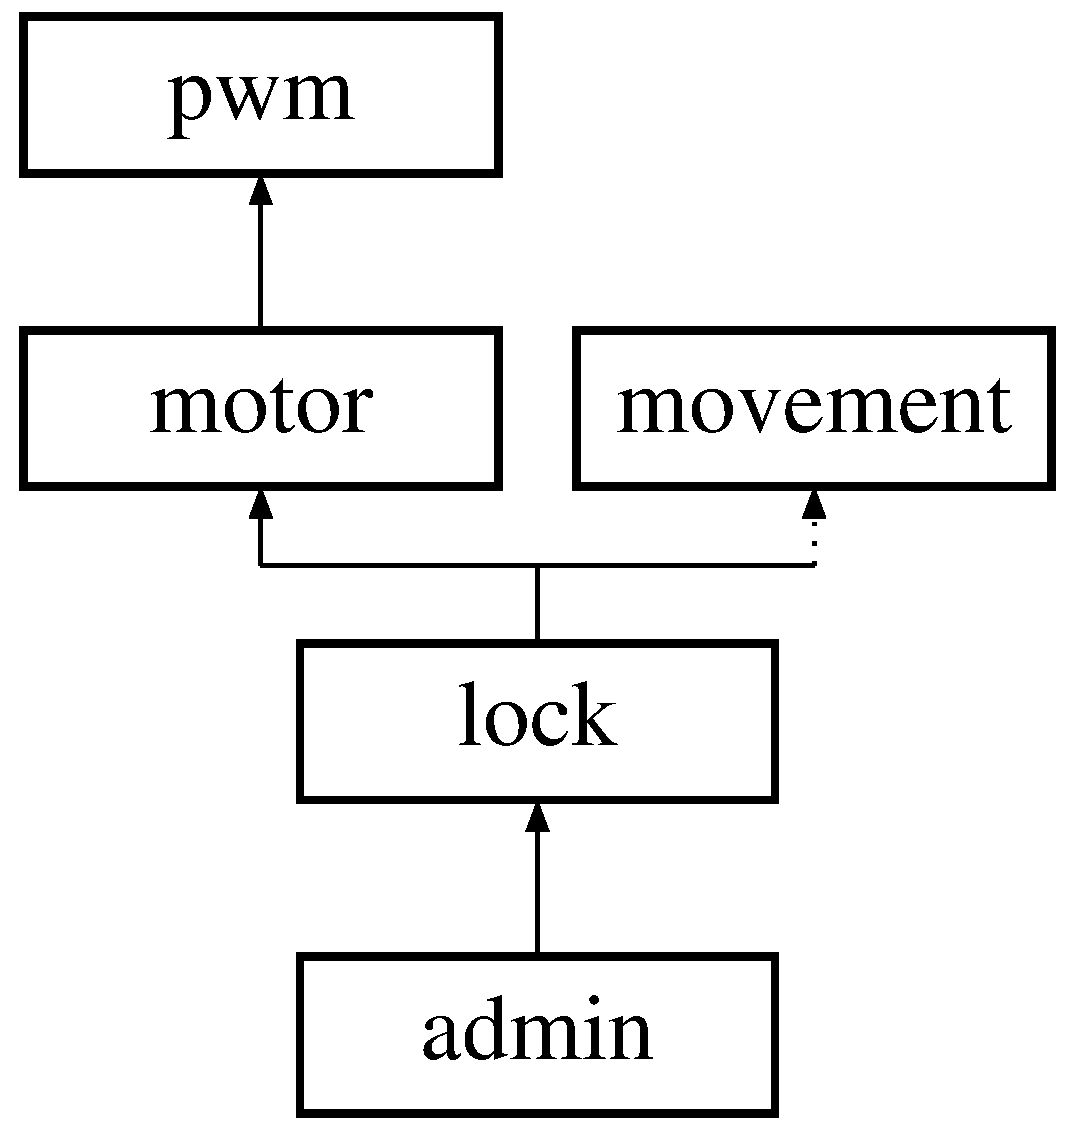
\includegraphics[height=4.000000cm]{classadmin}
\end{center}
\end{figure}
\subsection*{Public Member Functions}
\begin{DoxyCompactItemize}
\item 
{\bfseries admin} (\hyperlink{classlock}{lock} \&l, \hyperlink{classkeypad}{keypad} \&\hyperlink{classadmin_a945025347c265cad582b368ceca788c3}{k})\hypertarget{classadmin_a16cc376ed398bdf439973cacec5923ff}{}\label{classadmin_a16cc376ed398bdf439973cacec5923ff}

\item 
void \hyperlink{classadmin_a23a0137ba1609edd2f6b6f18eeaac975}{admin\+\_\+menu} ()
\begin{DoxyCompactList}\small\item\em admin\+\_\+menu function \end{DoxyCompactList}\item 
void \hyperlink{classadmin_a08aa886747be71f7916e8cc6c0806c2f}{admin\+\_\+wait} ()
\begin{DoxyCompactList}\small\item\em admin\+\_\+wait function \end{DoxyCompactList}\end{DoxyCompactItemize}
\subsection*{Protected Member Functions}
\begin{DoxyCompactItemize}
\item 
bool \hyperlink{classadmin_a20b580f1add145870f3b14944b4edf1a}{admin\+\_\+login} (\hyperlink{classpassword}{password} \&t)\hypertarget{classadmin_a20b580f1add145870f3b14944b4edf1a}{}\label{classadmin_a20b580f1add145870f3b14944b4edf1a}

\begin{DoxyCompactList}\small\item\em bool function for admin login \end{DoxyCompactList}\end{DoxyCompactItemize}
\subsection*{Protected Attributes}
\begin{DoxyCompactItemize}
\item 
\hyperlink{classpassword}{password} \hyperlink{classadmin_a1d06b76a2e4750d8c98472cb0ae30f4f}{p} = \hyperlink{classpassword}{password}(1,2,3,4)
\begin{DoxyCompactList}\small\item\em password p \end{DoxyCompactList}\item 
\hyperlink{classkeypad}{keypad} \& \hyperlink{classadmin_a945025347c265cad582b368ceca788c3}{k}\hypertarget{classadmin_a945025347c265cad582b368ceca788c3}{}\label{classadmin_a945025347c265cad582b368ceca788c3}

\begin{DoxyCompactList}\small\item\em reference to keypad \end{DoxyCompactList}\end{DoxyCompactItemize}


\subsection{Detailed Description}
class admin 

this class is an decorator for the soundlock class so it is possible to have different passwords on the same lock 

\subsection{Member Function Documentation}
\index{admin@{admin}!admin\+\_\+menu@{admin\+\_\+menu}}
\index{admin\+\_\+menu@{admin\+\_\+menu}!admin@{admin}}
\subsubsection[{\texorpdfstring{admin\+\_\+menu()}{admin_menu()}}]{\setlength{\rightskip}{0pt plus 5cm}void admin\+::admin\+\_\+menu (
\begin{DoxyParamCaption}
{}
\end{DoxyParamCaption}
)}\hypertarget{classadmin_a23a0137ba1609edd2f6b6f18eeaac975}{}\label{classadmin_a23a0137ba1609edd2f6b6f18eeaac975}


admin\+\_\+menu function 

this function is the menu for admin \index{admin@{admin}!admin\+\_\+wait@{admin\+\_\+wait}}
\index{admin\+\_\+wait@{admin\+\_\+wait}!admin@{admin}}
\subsubsection[{\texorpdfstring{admin\+\_\+wait()}{admin_wait()}}]{\setlength{\rightskip}{0pt plus 5cm}void admin\+::admin\+\_\+wait (
\begin{DoxyParamCaption}
{}
\end{DoxyParamCaption}
)}\hypertarget{classadmin_a08aa886747be71f7916e8cc6c0806c2f}{}\label{classadmin_a08aa886747be71f7916e8cc6c0806c2f}


admin\+\_\+wait function 

keep lock closed until password is put in 

\subsection{Member Data Documentation}
\index{admin@{admin}!p@{p}}
\index{p@{p}!admin@{admin}}
\subsubsection[{\texorpdfstring{p}{p}}]{\setlength{\rightskip}{0pt plus 5cm}{\bf password} admin\+::p = {\bf password}(1,2,3,4)\hspace{0.3cm}{\ttfamily [protected]}}\hypertarget{classadmin_a1d06b76a2e4750d8c98472cb0ae30f4f}{}\label{classadmin_a1d06b76a2e4750d8c98472cb0ae30f4f}


password p 

the password that belongs to the admin 

The documentation for this class was generated from the following files\+:\begin{DoxyCompactItemize}
\item 
admin.\+hpp\item 
admin.\+cpp\end{DoxyCompactItemize}

\hypertarget{classkeypad}{}\section{keypad Class Reference}
\label{classkeypad}\index{keypad@{keypad}}


keypad class  




{\ttfamily \#include $<$keypad.\+hpp$>$}

\subsection*{Public Member Functions}
\begin{DoxyCompactItemize}
\item 
\hyperlink{classkeypad_a6e342bf7c51143f25a84db9e0992039b}{keypad} (hwlib\+::target\+::pin\+\_\+out \&c1, hwlib\+::target\+::pin\+\_\+out \&c2, hwlib\+::target\+::pin\+\_\+out \&c3, hwlib\+::target\+::pin\+\_\+out \&c4, hwlib\+::target\+::pin\+\_\+in \&r1, hwlib\+::target\+::pin\+\_\+in \&r2, hwlib\+::target\+::pin\+\_\+in \&r3, hwlib\+::target\+::pin\+\_\+in \&r4)
\begin{DoxyCompactList}\small\item\em the default constructor \end{DoxyCompactList}\item 
int \hyperlink{classkeypad_a2a1334d93f32abfe59930a35b61bdbba}{input} ()
\begin{DoxyCompactList}\small\item\em int input function. \end{DoxyCompactList}\end{DoxyCompactItemize}


\subsection{Detailed Description}
keypad class 

class for the reading of an 4x4 matrix keypad 

\subsection{Constructor \& Destructor Documentation}
\index{keypad@{keypad}!keypad@{keypad}}
\index{keypad@{keypad}!keypad@{keypad}}
\subsubsection[{\texorpdfstring{keypad(hwlib\+::target\+::pin\+\_\+out \&c1, hwlib\+::target\+::pin\+\_\+out \&c2, hwlib\+::target\+::pin\+\_\+out \&c3, hwlib\+::target\+::pin\+\_\+out \&c4, hwlib\+::target\+::pin\+\_\+in \&r1, hwlib\+::target\+::pin\+\_\+in \&r2, hwlib\+::target\+::pin\+\_\+in \&r3, hwlib\+::target\+::pin\+\_\+in \&r4)}{keypad(hwlib::target::pin_out &c1, hwlib::target::pin_out &c2, hwlib::target::pin_out &c3, hwlib::target::pin_out &c4, hwlib::target::pin_in &r1, hwlib::target::pin_in &r2, hwlib::target::pin_in &r3, hwlib::target::pin_in &r4)}}]{\setlength{\rightskip}{0pt plus 5cm}keypad\+::keypad (
\begin{DoxyParamCaption}
\item[{hwlib\+::target\+::pin\+\_\+out \&}]{c1, }
\item[{hwlib\+::target\+::pin\+\_\+out \&}]{c2, }
\item[{hwlib\+::target\+::pin\+\_\+out \&}]{c3, }
\item[{hwlib\+::target\+::pin\+\_\+out \&}]{c4, }
\item[{hwlib\+::target\+::pin\+\_\+in \&}]{r1, }
\item[{hwlib\+::target\+::pin\+\_\+in \&}]{r2, }
\item[{hwlib\+::target\+::pin\+\_\+in \&}]{r3, }
\item[{hwlib\+::target\+::pin\+\_\+in \&}]{r4}
\end{DoxyParamCaption}
)}\hypertarget{classkeypad_a6e342bf7c51143f25a84db9e0992039b}{}\label{classkeypad_a6e342bf7c51143f25a84db9e0992039b}


the default constructor 

the constructor gets eigth pins in referrence four pins are input and four pins are output. 

\subsection{Member Function Documentation}
\index{keypad@{keypad}!input@{input}}
\index{input@{input}!keypad@{keypad}}
\subsubsection[{\texorpdfstring{input()}{input()}}]{\setlength{\rightskip}{0pt plus 5cm}int keypad\+::input (
\begin{DoxyParamCaption}
{}
\end{DoxyParamCaption}
)}\hypertarget{classkeypad_a2a1334d93f32abfe59930a35b61bdbba}{}\label{classkeypad_a2a1334d93f32abfe59930a35b61bdbba}


int input function. 

gives the value back that the position contains out the matrix that is equal to the position that is pressed. 

The documentation for this class was generated from the following files\+:\begin{DoxyCompactItemize}
\item 
keypad.\+hpp\item 
keypad.\+cpp\end{DoxyCompactItemize}

\hypertarget{classlock}{}\section{lock Class Reference}
\label{classlock}\index{lock@{lock}}


lock class  




{\ttfamily \#include $<$lock.\+hpp$>$}

\subsection*{Public Member Functions}
\begin{DoxyCompactItemize}
\item 
\hyperlink{classlock_a70661afaf29f414bf0b838dfbc9c10a6}{lock} (hwlib\+::target\+::pin\+\_\+out \&pinout, hwlib\+::target\+::pin\+\_\+in \&pinin)
\begin{DoxyCompactList}\small\item\em default constructor \end{DoxyCompactList}\item 
virtual void \hyperlink{classlock_a773859340b99fff94e8a21206d5906bd}{open} ()
\begin{DoxyCompactList}\small\item\em virtual open function \end{DoxyCompactList}\item 
virtual void \hyperlink{classlock_a7e4aac202a1b73f57338ea7f935cf9ce}{close} ()
\begin{DoxyCompactList}\small\item\em virtual close function \end{DoxyCompactList}\item 
void \hyperlink{classlock_a1e203e71ff7300d4202516c1b08c3ad2}{pir} ()
\begin{DoxyCompactList}\small\item\em pir function \end{DoxyCompactList}\end{DoxyCompactItemize}


\subsection{Detailed Description}
lock class 

lock class combine motor class (servo) with movement class(pir) 

\subsection{Constructor \& Destructor Documentation}
\index{lock@{lock}!lock@{lock}}
\index{lock@{lock}!lock@{lock}}
\subsubsection[{\texorpdfstring{lock(hwlib\+::target\+::pin\+\_\+out \&pinout, hwlib\+::target\+::pin\+\_\+in \&pinin)}{lock(hwlib::target::pin_out &pinout, hwlib::target::pin_in &pinin)}}]{\setlength{\rightskip}{0pt plus 5cm}lock\+::lock (
\begin{DoxyParamCaption}
\item[{hwlib\+::target\+::pin\+\_\+out \&}]{pinout, }
\item[{hwlib\+::target\+::pin\+\_\+in \&}]{pinin}
\end{DoxyParamCaption}
)}\hypertarget{classlock_a70661afaf29f414bf0b838dfbc9c10a6}{}\label{classlock_a70661afaf29f414bf0b838dfbc9c10a6}


default constructor 

the constructor gets a pin\+\_\+out reference for the motor (move) and a pin\+\_\+in reference for the movement (see). 

\subsection{Member Function Documentation}
\index{lock@{lock}!close@{close}}
\index{close@{close}!lock@{lock}}
\subsubsection[{\texorpdfstring{close()}{close()}}]{\setlength{\rightskip}{0pt plus 5cm}void lock\+::close (
\begin{DoxyParamCaption}
{}
\end{DoxyParamCaption}
)\hspace{0.3cm}{\ttfamily [virtual]}}\hypertarget{classlock_a7e4aac202a1b73f57338ea7f935cf9ce}{}\label{classlock_a7e4aac202a1b73f57338ea7f935cf9ce}


virtual close function 

default \+: this function closes the lock if the lock is open . it turns the motor to 90 degrees by using the turnto90 function. the function is virtual so it is possible to have an different set up with the lock \index{lock@{lock}!open@{open}}
\index{open@{open}!lock@{lock}}
\subsubsection[{\texorpdfstring{open()}{open()}}]{\setlength{\rightskip}{0pt plus 5cm}void lock\+::open (
\begin{DoxyParamCaption}
{}
\end{DoxyParamCaption}
)\hspace{0.3cm}{\ttfamily [virtual]}}\hypertarget{classlock_a773859340b99fff94e8a21206d5906bd}{}\label{classlock_a773859340b99fff94e8a21206d5906bd}


virtual open function 

this function opens the lock if the lock is closed . it turns the motor to 0 degrees by using the turnto0 function. the function is virtual so it is possible to have an different set up with the lock \index{lock@{lock}!pir@{pir}}
\index{pir@{pir}!lock@{lock}}
\subsubsection[{\texorpdfstring{pir()}{pir()}}]{\setlength{\rightskip}{0pt plus 5cm}void lock\+::pir (
\begin{DoxyParamCaption}
{}
\end{DoxyParamCaption}
)}\hypertarget{classlock_a1e203e71ff7300d4202516c1b08c3ad2}{}\label{classlock_a1e203e71ff7300d4202516c1b08c3ad2}


pir function 

this function closes the lock when someone is moving by and if the lock is open at that moment 

The documentation for this class was generated from the following files\+:\begin{DoxyCompactItemize}
\item 
lock.\+hpp\item 
lock.\+cpp\end{DoxyCompactItemize}

\hypertarget{classmotor}{}\section{motor Class Reference}
\label{classmotor}\index{motor@{motor}}


class for control of 9g\+\_\+servo  




{\ttfamily \#include $<$motor\+\_\+g9.\+hpp$>$}

Inheritance diagram for motor\+:\begin{figure}[H]
\begin{center}
\leavevmode
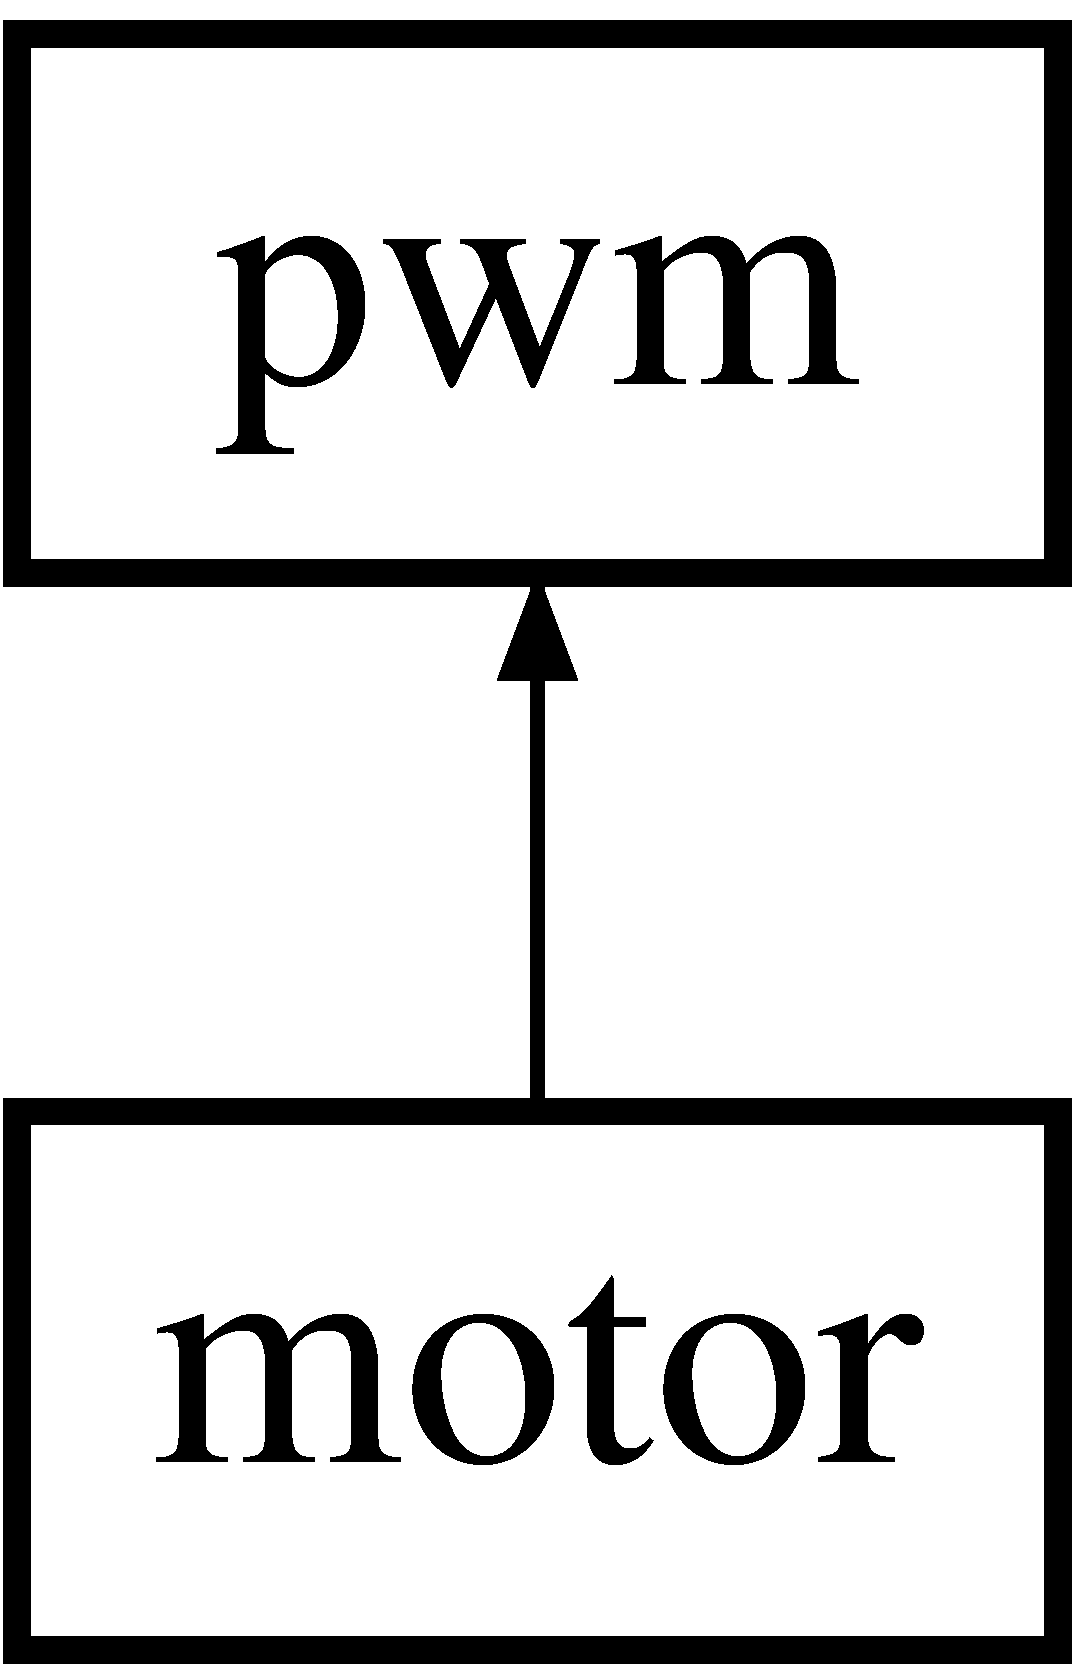
\includegraphics[height=4.000000cm]{classmotor}
\end{center}
\end{figure}
\subsection*{Public Member Functions}
\begin{DoxyCompactItemize}
\item 
\hyperlink{classmotor_a2a03c0b137ceaf886d406f55bc1dfc6d}{motor} (hwlib\+::target\+::pin\+\_\+out \&pwmpin)
\begin{DoxyCompactList}\small\item\em default constructor \end{DoxyCompactList}\item 
void \hyperlink{classmotor_a4d056e4f75a5613ef50a4ae4ed95525d}{turn} (int degrees)
\begin{DoxyCompactList}\small\item\em turn the servo to an desired amount of degrees. \end{DoxyCompactList}\item 
void \hyperlink{classmotor_a942b9474ad3226a035908333d5d09a86}{turnto0} ()
\begin{DoxyCompactList}\small\item\em turnto0 function \end{DoxyCompactList}\item 
void \hyperlink{classmotor_a8983111ce2a6fb60d1ef4d26028981c8}{turnto90} ()
\begin{DoxyCompactList}\small\item\em turnto0 function \end{DoxyCompactList}\end{DoxyCompactItemize}


\subsection{Detailed Description}
class for control of 9g\+\_\+servo 

this class is an decorator class to the pwm class in this class the pulse function is used to create the signal used for the \hyperlink{classservo}{servo( 9g analog)} 

\subsection{Constructor \& Destructor Documentation}
\index{motor@{motor}!motor@{motor}}
\index{motor@{motor}!motor@{motor}}
\subsubsection[{\texorpdfstring{motor(hwlib\+::target\+::pin\+\_\+out \&pwmpin)}{motor(hwlib::target::pin_out &pwmpin)}}]{\setlength{\rightskip}{0pt plus 5cm}motor\+::motor (
\begin{DoxyParamCaption}
\item[{hwlib\+::target\+::pin\+\_\+out \&}]{pwmpin}
\end{DoxyParamCaption}
)}\hypertarget{classmotor_a2a03c0b137ceaf886d406f55bc1dfc6d}{}\label{classmotor_a2a03c0b137ceaf886d406f55bc1dfc6d}


default constructor 

the constructor gets an reference to the ouput pin used for the pwm signal used for the servo 

\subsection{Member Function Documentation}
\index{motor@{motor}!turn@{turn}}
\index{turn@{turn}!motor@{motor}}
\subsubsection[{\texorpdfstring{turn(int degrees)}{turn(int degrees)}}]{\setlength{\rightskip}{0pt plus 5cm}void motor\+::turn (
\begin{DoxyParamCaption}
\item[{int}]{degrees}
\end{DoxyParamCaption}
)}\hypertarget{classmotor_a4d056e4f75a5613ef50a4ae4ed95525d}{}\label{classmotor_a4d056e4f75a5613ef50a4ae4ed95525d}


turn the servo to an desired amount of degrees. 

turn function gets an amount of degrees and calculates the correct value for the wait in the pulse function \index{motor@{motor}!turnto0@{turnto0}}
\index{turnto0@{turnto0}!motor@{motor}}
\subsubsection[{\texorpdfstring{turnto0()}{turnto0()}}]{\setlength{\rightskip}{0pt plus 5cm}void motor\+::turnto0 (
\begin{DoxyParamCaption}
{}
\end{DoxyParamCaption}
)}\hypertarget{classmotor_a942b9474ad3226a035908333d5d09a86}{}\label{classmotor_a942b9474ad3226a035908333d5d09a86}


turnto0 function 

this function uses the turn function and is pre set to turn the servo to 0 degrees in contrast to the turnto90 function \index{motor@{motor}!turnto90@{turnto90}}
\index{turnto90@{turnto90}!motor@{motor}}
\subsubsection[{\texorpdfstring{turnto90()}{turnto90()}}]{\setlength{\rightskip}{0pt plus 5cm}void motor\+::turnto90 (
\begin{DoxyParamCaption}
{}
\end{DoxyParamCaption}
)}\hypertarget{classmotor_a8983111ce2a6fb60d1ef4d26028981c8}{}\label{classmotor_a8983111ce2a6fb60d1ef4d26028981c8}


turnto0 function 

this function uses the turn function and is pre set to turn the servo to 90 degree in contrast to the turnto0 function 

The documentation for this class was generated from the following files\+:\begin{DoxyCompactItemize}
\item 
motor\+\_\+g9.\+hpp\item 
motor\+\_\+g9.\+cpp\end{DoxyCompactItemize}

\hypertarget{classmovement}{}\section{movement Class Reference}
\label{classmovement}\index{movement@{movement}}


class for the pir sensor  




{\ttfamily \#include $<$movement.\+hpp$>$}

\subsection*{Public Member Functions}
\begin{DoxyCompactItemize}
\item 
\hyperlink{classmovement_a4dd6685da16ddabc964ce08f71bb4ff1}{movement} (hwlib\+::target\+::pin\+\_\+in \&pir)
\begin{DoxyCompactList}\small\item\em the construtor of the movement class needs one input pin for the pir \end{DoxyCompactList}\item 
bool \hyperlink{classmovement_a67f9250eec2b5628cf6e41d5f1f5ef30}{get} ()
\begin{DoxyCompactList}\small\item\em function getis for getting the value of the pir sensor. \end{DoxyCompactList}\end{DoxyCompactItemize}


\subsection{Detailed Description}
class for the pir sensor 

\subsection{Constructor \& Destructor Documentation}
\index{movement@{movement}!movement@{movement}}
\index{movement@{movement}!movement@{movement}}
\subsubsection[{\texorpdfstring{movement(hwlib\+::target\+::pin\+\_\+in \&pir)}{movement(hwlib::target::pin_in &pir)}}]{\setlength{\rightskip}{0pt plus 5cm}movement\+::movement (
\begin{DoxyParamCaption}
\item[{hwlib\+::target\+::pin\+\_\+in \&}]{pir}
\end{DoxyParamCaption}
)}\hypertarget{classmovement_a4dd6685da16ddabc964ce08f71bb4ff1}{}\label{classmovement_a4dd6685da16ddabc964ce08f71bb4ff1}


the construtor of the movement class needs one input pin for the pir 

movement constructor needs one input pin used for the pir sensor 

\subsection{Member Function Documentation}
\index{movement@{movement}!get@{get}}
\index{get@{get}!movement@{movement}}
\subsubsection[{\texorpdfstring{get()}{get()}}]{\setlength{\rightskip}{0pt plus 5cm}bool movement\+::get (
\begin{DoxyParamCaption}
{}
\end{DoxyParamCaption}
)}\hypertarget{classmovement_a67f9250eec2b5628cf6e41d5f1f5ef30}{}\label{classmovement_a67f9250eec2b5628cf6e41d5f1f5ef30}


function getis for getting the value of the pir sensor. 

get function returns the value the pir sensor is giving 

The documentation for this class was generated from the following files\+:\begin{DoxyCompactItemize}
\item 
movement.\+hpp\item 
movement.\+cpp\end{DoxyCompactItemize}

\hypertarget{classpassword}{}\section{password Class Reference}
\label{classpassword}\index{password@{password}}


password A\+DT  




{\ttfamily \#include $<$password.\+hpp$>$}

\subsection*{Public Member Functions}
\begin{DoxyCompactItemize}
\item 
\hyperlink{classpassword_a73408df5e3c516dfe53b968ac700d18d}{password} (int \hyperlink{classpassword_a0e2e6d171003a3a8594a2cfec2b9c059}{tel876}, int \hyperlink{classpassword_ad5afb40aeb150953f66a1c14745297bc}{tel54}, int \hyperlink{classpassword_a93ef3ccb4e71a683115c12435c89411d}{tel32}, int \hyperlink{classpassword_af09c363ed2ec22c8e900fdd6bf66c1f6}{tel10})
\begin{DoxyCompactList}\small\item\em default constructor \end{DoxyCompactList}\item 
\hyperlink{classpassword_aa9dba4c6670c6e2e848b16f036865c54}{password} ()
\begin{DoxyCompactList}\small\item\em empty constructor \end{DoxyCompactList}\item 
void \hyperlink{classpassword_a107a4017891e000323e7300b0d67ba20}{operator=} (const \hyperlink{classpassword}{password} \&rhs)
\begin{DoxyCompactList}\small\item\em = operator \end{DoxyCompactList}\item 
\hyperlink{classpassword}{password} \hyperlink{classpassword_a319c42d6fcfe0f7e36999a00a6bdd4a0}{operator+} (const \hyperlink{classpassword}{password} \&rhs) const 
\begin{DoxyCompactList}\small\item\em this operator sum two passwords \end{DoxyCompactList}\item 
\hyperlink{classpassword}{password} \hyperlink{classpassword_a1d15ab4bff819d61b48b0b2835b40afa}{operator/} (const int rhs) const 
\begin{DoxyCompactList}\small\item\em / operator \end{DoxyCompactList}\item 
\hyperlink{classpassword}{password} \hyperlink{classpassword_a775500307f55707d950c6605de07c400}{operator$\ast$} (const int rhs) const 
\begin{DoxyCompactList}\small\item\em this operator multiplies an password with an integer \end{DoxyCompactList}\item 
bool \hyperlink{classpassword_a528a04105bb089391277c217d8272462}{operator==} (const \hyperlink{classpassword}{password} \&rhs) const 
\begin{DoxyCompactList}\small\item\em bool == operator \end{DoxyCompactList}\item 
bool \hyperlink{classpassword_aa15f528d4cdd5da15d5ea29b9cbe586f}{operator$>$=} (const \hyperlink{classpassword}{password} \&rhs) const 
\begin{DoxyCompactList}\small\item\em bool == operator \end{DoxyCompactList}\item 
\hyperlink{classpassword}{password} \& \hyperlink{classpassword_a5c4a32e2761f6d35ddd7d633955e6b0e}{operator+=} (const \hyperlink{classpassword}{password} \&rhs)
\begin{DoxyCompactList}\small\item\em += operator \end{DoxyCompactList}\end{DoxyCompactItemize}
\subsection*{Protected Attributes}
\begin{DoxyCompactItemize}
\item 
int \hyperlink{classpassword_a0e2e6d171003a3a8594a2cfec2b9c059}{tel876}
\begin{DoxyCompactList}\small\item\em integer tel876 \end{DoxyCompactList}\item 
int \hyperlink{classpassword_ad5afb40aeb150953f66a1c14745297bc}{tel54}
\begin{DoxyCompactList}\small\item\em integer tel54 \end{DoxyCompactList}\item 
int \hyperlink{classpassword_a93ef3ccb4e71a683115c12435c89411d}{tel32}
\begin{DoxyCompactList}\small\item\em integer tel32 \end{DoxyCompactList}\item 
int \hyperlink{classpassword_af09c363ed2ec22c8e900fdd6bf66c1f6}{tel10}
\begin{DoxyCompactList}\small\item\em integer tel10 \end{DoxyCompactList}\end{DoxyCompactItemize}
\subsection*{Friends}
\begin{DoxyCompactItemize}
\item 
hwlib\+::ostream \& \hyperlink{classpassword_a8ce6de07d3729f31df4476763ca155ca}{operator$<$$<$} (hwlib\+::ostream \&lhs, const \hyperlink{classpassword}{password} \&rhs)
\begin{DoxyCompactList}\small\item\em hwlib\+::ostream $<$$<$ operator \end{DoxyCompactList}\end{DoxyCompactItemize}


\subsection{Detailed Description}
password A\+DT 

this is an A\+DT that saves the passwords. this A\+DT contains four integers. that are beeing used in this library. 

\subsection{Constructor \& Destructor Documentation}
\index{password@{password}!password@{password}}
\index{password@{password}!password@{password}}
\subsubsection[{\texorpdfstring{password(int tel876, int tel54, int tel32, int tel10)}{password(int tel876, int tel54, int tel32, int tel10)}}]{\setlength{\rightskip}{0pt plus 5cm}password\+::password (
\begin{DoxyParamCaption}
\item[{int}]{tel876, }
\item[{int}]{tel54, }
\item[{int}]{tel32, }
\item[{int}]{tel10}
\end{DoxyParamCaption}
)}\hypertarget{classpassword_a73408df5e3c516dfe53b968ac700d18d}{}\label{classpassword_a73408df5e3c516dfe53b968ac700d18d}


default constructor 

this constructor gets 4 integers that are stalled as password \index{password@{password}!password@{password}}
\index{password@{password}!password@{password}}
\subsubsection[{\texorpdfstring{password()}{password()}}]{\setlength{\rightskip}{0pt plus 5cm}password\+::password (
\begin{DoxyParamCaption}
{}
\end{DoxyParamCaption}
)}\hypertarget{classpassword_aa9dba4c6670c6e2e848b16f036865c54}{}\label{classpassword_aa9dba4c6670c6e2e848b16f036865c54}


empty constructor 

when an password has to be still calculated and/or determend the values will stay empty (used in profile class) 

\subsection{Member Function Documentation}
\index{password@{password}!operator$\ast$@{operator$\ast$}}
\index{operator$\ast$@{operator$\ast$}!password@{password}}
\subsubsection[{\texorpdfstring{operator$\ast$(const int rhs) const }{operator*(const int rhs) const }}]{\setlength{\rightskip}{0pt plus 5cm}{\bf password} password\+::operator$\ast$ (
\begin{DoxyParamCaption}
\item[{const int}]{rhs}
\end{DoxyParamCaption}
) const}\hypertarget{classpassword_a775500307f55707d950c6605de07c400}{}\label{classpassword_a775500307f55707d950c6605de07c400}


this operator multiplies an password with an integer 


\begin{DoxyItemize}
\item operator 
\end{DoxyItemize}\index{password@{password}!operator+@{operator+}}
\index{operator+@{operator+}!password@{password}}
\subsubsection[{\texorpdfstring{operator+(const password \&rhs) const }{operator+(const password &rhs) const }}]{\setlength{\rightskip}{0pt plus 5cm}{\bf password} password\+::operator+ (
\begin{DoxyParamCaption}
\item[{const {\bf password} \&}]{rhs}
\end{DoxyParamCaption}
) const}\hypertarget{classpassword_a319c42d6fcfe0f7e36999a00a6bdd4a0}{}\label{classpassword_a319c42d6fcfe0f7e36999a00a6bdd4a0}


this operator sum two passwords 


\begin{DoxyItemize}
\item operator 
\end{DoxyItemize}\index{password@{password}!operator+=@{operator+=}}
\index{operator+=@{operator+=}!password@{password}}
\subsubsection[{\texorpdfstring{operator+=(const password \&rhs)}{operator+=(const password &rhs)}}]{\setlength{\rightskip}{0pt plus 5cm}{\bf password} \& password\+::operator+= (
\begin{DoxyParamCaption}
\item[{const {\bf password} \&}]{rhs}
\end{DoxyParamCaption}
)}\hypertarget{classpassword_a5c4a32e2761f6d35ddd7d633955e6b0e}{}\label{classpassword_a5c4a32e2761f6d35ddd7d633955e6b0e}


+= operator 

this operator adds an password to an other password \index{password@{password}!operator/@{operator/}}
\index{operator/@{operator/}!password@{password}}
\subsubsection[{\texorpdfstring{operator/(const int rhs) const }{operator/(const int rhs) const }}]{\setlength{\rightskip}{0pt plus 5cm}{\bf password} password\+::operator/ (
\begin{DoxyParamCaption}
\item[{const int}]{rhs}
\end{DoxyParamCaption}
) const}\hypertarget{classpassword_a1d15ab4bff819d61b48b0b2835b40afa}{}\label{classpassword_a1d15ab4bff819d61b48b0b2835b40afa}


/ operator 

this oprator divide an password with an integer. \index{password@{password}!operator=@{operator=}}
\index{operator=@{operator=}!password@{password}}
\subsubsection[{\texorpdfstring{operator=(const password \&rhs)}{operator=(const password &rhs)}}]{\setlength{\rightskip}{0pt plus 5cm}void password\+::operator= (
\begin{DoxyParamCaption}
\item[{const {\bf password} \&}]{rhs}
\end{DoxyParamCaption}
)}\hypertarget{classpassword_a107a4017891e000323e7300b0d67ba20}{}\label{classpassword_a107a4017891e000323e7300b0d67ba20}


= operator 

this operator makes it possile to give an password the values of an other password. for example when an password is empty and the calculation is done it can e put in the correct please (used in set\+\_\+pasword function in profile class) \index{password@{password}!operator==@{operator==}}
\index{operator==@{operator==}!password@{password}}
\subsubsection[{\texorpdfstring{operator==(const password \&rhs) const }{operator==(const password &rhs) const }}]{\setlength{\rightskip}{0pt plus 5cm}bool password\+::operator== (
\begin{DoxyParamCaption}
\item[{const {\bf password} \&}]{rhs}
\end{DoxyParamCaption}
) const}\hypertarget{classpassword_a528a04105bb089391277c217d8272462}{}\label{classpassword_a528a04105bb089391277c217d8272462}


bool == operator 

this bool operator compares two passwords with an certain marge \index{password@{password}!operator$>$=@{operator$>$=}}
\index{operator$>$=@{operator$>$=}!password@{password}}
\subsubsection[{\texorpdfstring{operator$>$=(const password \&rhs) const }{operator>=(const password &rhs) const }}]{\setlength{\rightskip}{0pt plus 5cm}bool password\+::operator$>$= (
\begin{DoxyParamCaption}
\item[{const {\bf password} \&}]{rhs}
\end{DoxyParamCaption}
) const}\hypertarget{classpassword_aa15f528d4cdd5da15d5ea29b9cbe586f}{}\label{classpassword_aa15f528d4cdd5da15d5ea29b9cbe586f}


bool == operator 

this bool operator compares two passwords without marge. 

\subsection{Friends And Related Function Documentation}
\index{password@{password}!operator$<$$<$@{operator$<$$<$}}
\index{operator$<$$<$@{operator$<$$<$}!password@{password}}
\subsubsection[{\texorpdfstring{operator$<$$<$}{operator<<}}]{\setlength{\rightskip}{0pt plus 5cm}hwlib\+::ostream\& operator$<$$<$ (
\begin{DoxyParamCaption}
\item[{hwlib\+::ostream \&}]{lhs, }
\item[{const {\bf password} \&}]{rhs}
\end{DoxyParamCaption}
)\hspace{0.3cm}{\ttfamily [friend]}}\hypertarget{classpassword_a8ce6de07d3729f31df4476763ca155ca}{}\label{classpassword_a8ce6de07d3729f31df4476763ca155ca}


hwlib\+::ostream $<$$<$ operator 

makes it possible to print out an password to the terminal 

\subsection{Member Data Documentation}
\index{password@{password}!tel10@{tel10}}
\index{tel10@{tel10}!password@{password}}
\subsubsection[{\texorpdfstring{tel10}{tel10}}]{\setlength{\rightskip}{0pt plus 5cm}int password\+::tel10\hspace{0.3cm}{\ttfamily [protected]}}\hypertarget{classpassword_af09c363ed2ec22c8e900fdd6bf66c1f6}{}\label{classpassword_af09c363ed2ec22c8e900fdd6bf66c1f6}


integer tel10 

this integer is first of the four numbers of an password . it is determinate in the math\+\_\+password function. \index{password@{password}!tel32@{tel32}}
\index{tel32@{tel32}!password@{password}}
\subsubsection[{\texorpdfstring{tel32}{tel32}}]{\setlength{\rightskip}{0pt plus 5cm}int password\+::tel32\hspace{0.3cm}{\ttfamily [protected]}}\hypertarget{classpassword_a93ef3ccb4e71a683115c12435c89411d}{}\label{classpassword_a93ef3ccb4e71a683115c12435c89411d}


integer tel32 

this integer is third of the four numbers of an password . it is determinate in the math\+\_\+password function. \index{password@{password}!tel54@{tel54}}
\index{tel54@{tel54}!password@{password}}
\subsubsection[{\texorpdfstring{tel54}{tel54}}]{\setlength{\rightskip}{0pt plus 5cm}int password\+::tel54\hspace{0.3cm}{\ttfamily [protected]}}\hypertarget{classpassword_ad5afb40aeb150953f66a1c14745297bc}{}\label{classpassword_ad5afb40aeb150953f66a1c14745297bc}


integer tel54 

this integer is second of the four numbers of an password . it is determinate in the math\+\_\+password function. \index{password@{password}!tel876@{tel876}}
\index{tel876@{tel876}!password@{password}}
\subsubsection[{\texorpdfstring{tel876}{tel876}}]{\setlength{\rightskip}{0pt plus 5cm}int password\+::tel876\hspace{0.3cm}{\ttfamily [protected]}}\hypertarget{classpassword_a0e2e6d171003a3a8594a2cfec2b9c059}{}\label{classpassword_a0e2e6d171003a3a8594a2cfec2b9c059}


integer tel876 

this integer is first of the four numbers of an password . it is determinate in the math\+\_\+password function. 

The documentation for this class was generated from the following files\+:\begin{DoxyCompactItemize}
\item 
password.\+hpp\item 
password.\+cpp\end{DoxyCompactItemize}

\hypertarget{classprofile}{}\section{profile Class Reference}
\label{classprofile}\index{profile@{profile}}


class profile  




{\ttfamily \#include $<$profile.\+hpp$>$}

Inheritance diagram for profile\+:\begin{figure}[H]
\begin{center}
\leavevmode
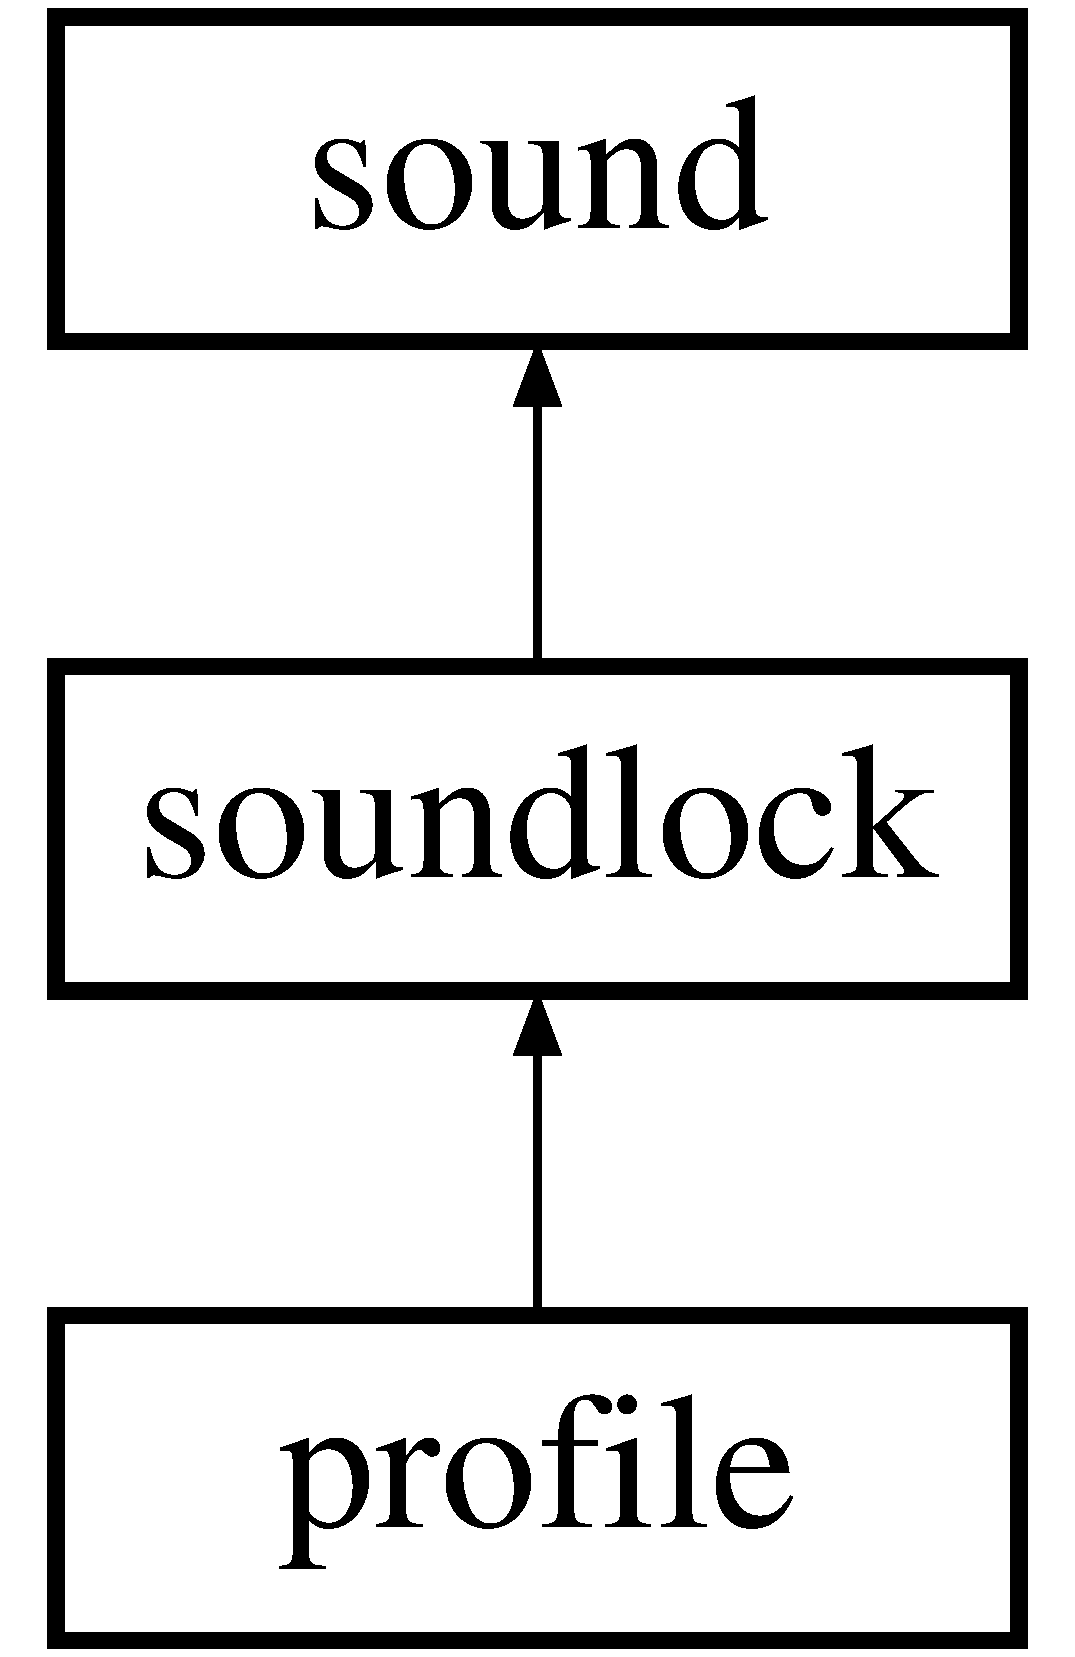
\includegraphics[height=3.000000cm]{classprofile}
\end{center}
\end{figure}
\subsection*{Public Member Functions}
\begin{DoxyCompactItemize}
\item 
\hyperlink{classprofile_aa556404d805d160561f593b02789c5d6}{profile} (hwlib\+::target\+::pin\+\_\+adc \&\hyperlink{classsound_a1b4c38e994daa1b3e9006852d3d9242a}{adc}, \hyperlink{classlock}{lock} \&\hyperlink{classsoundlock_ade415e22f230dca2d7e7f93d14cec8b6}{l})
\begin{DoxyCompactList}\small\item\em default constructor \end{DoxyCompactList}\item 
void \hyperlink{classprofile_acefbce03d19dafccbcf55c17b3527a23}{compare\+\_\+password} () override
\begin{DoxyCompactList}\small\item\em function compare\+\_\+password \end{DoxyCompactList}\end{DoxyCompactItemize}
\subsection*{Protected Member Functions}
\begin{DoxyCompactItemize}
\item 
void \hyperlink{classprofile_aa46b5ea874a915a76a54c4ce7fa9701c}{set\+\_\+password} () override
\begin{DoxyCompactList}\small\item\em function set\+\_\+password \end{DoxyCompactList}\item 
void \hyperlink{classprofile_a85a7931430f0cc2abc94253548b9cb37}{math\+\_\+password} () override
\begin{DoxyCompactList}\small\item\em funtion math\+\_\+password \end{DoxyCompactList}\item 
void \hyperlink{classprofile_a5cd64e12649b049cfee501c2e976bd96}{measure} () override
\begin{DoxyCompactList}\small\item\em funcion measure \end{DoxyCompactList}\end{DoxyCompactItemize}
\subsection*{Protected Attributes}
\begin{DoxyCompactItemize}
\item 
\hyperlink{classpassword}{password} \hyperlink{classprofile_afbf1e7946aa806c96044b94349a4bdad}{p}
\begin{DoxyCompactList}\small\item\em password p \end{DoxyCompactList}\item 
bool \hyperlink{classprofile_a82b3f6d034c00c6e180a3df4c46ce0f8}{set\+\_\+p} =0
\begin{DoxyCompactList}\small\item\em bool set\+\_\+p \end{DoxyCompactList}\item 
bool \hyperlink{classprofile_a0a35d68e263091faa4f4855f27ef3f38}{set\+\_\+p\+\_\+run} =0
\begin{DoxyCompactList}\small\item\em bool set\+\_\+p\+\_\+run \end{DoxyCompactList}\end{DoxyCompactItemize}


\subsection{Detailed Description}
class profile 

this class is an decorator for the soundlock class so it is possible to have different passwords on the same lock 

\subsection{Constructor \& Destructor Documentation}
\index{profile@{profile}!profile@{profile}}
\index{profile@{profile}!profile@{profile}}
\subsubsection[{\texorpdfstring{profile(hwlib\+::target\+::pin\+\_\+adc \&adc, lock \&l)}{profile(hwlib::target::pin_adc &adc, lock &l)}}]{\setlength{\rightskip}{0pt plus 5cm}profile\+::profile (
\begin{DoxyParamCaption}
\item[{hwlib\+::target\+::pin\+\_\+adc \&}]{adc, }
\item[{{\bf lock} \&}]{l}
\end{DoxyParamCaption}
)}\hypertarget{classprofile_aa556404d805d160561f593b02789c5d6}{}\label{classprofile_aa556404d805d160561f593b02789c5d6}


default constructor 

the constuctor gets an reference to an analog pin used for analog to digital conversion and anreference to an lock needed for the soundlock function. 

\subsection{Member Function Documentation}
\index{profile@{profile}!compare\+\_\+password@{compare\+\_\+password}}
\index{compare\+\_\+password@{compare\+\_\+password}!profile@{profile}}
\subsubsection[{\texorpdfstring{compare\+\_\+password() override}{compare_password() override}}]{\setlength{\rightskip}{0pt plus 5cm}void profile\+::compare\+\_\+password (
\begin{DoxyParamCaption}
{}
\end{DoxyParamCaption}
)\hspace{0.3cm}{\ttfamily [override]}, {\ttfamily [virtual]}}\hypertarget{classprofile_acefbce03d19dafccbcf55c17b3527a23}{}\label{classprofile_acefbce03d19dafccbcf55c17b3527a23}


function compare\+\_\+password 

this function is the override for the virtual compare \+\_\+password function in soundlock this function compares the temp password with the set password p. if there isn\textquotesingle{}t set an password then it redirect to set\+\_\+password function 

Implements \hyperlink{classsoundlock_abca4638dd9dd78157c2c18165407965e}{soundlock}.

\index{profile@{profile}!math\+\_\+password@{math\+\_\+password}}
\index{math\+\_\+password@{math\+\_\+password}!profile@{profile}}
\subsubsection[{\texorpdfstring{math\+\_\+password() override}{math_password() override}}]{\setlength{\rightskip}{0pt plus 5cm}void profile\+::math\+\_\+password (
\begin{DoxyParamCaption}
{}
\end{DoxyParamCaption}
)\hspace{0.3cm}{\ttfamily [override]}, {\ttfamily [protected]}, {\ttfamily [virtual]}}\hypertarget{classprofile_a85a7931430f0cc2abc94253548b9cb37}{}\label{classprofile_a85a7931430f0cc2abc94253548b9cb37}


funtion math\+\_\+password 

this function is the override for the virtual math \+\_\+password function in soundlock the calculation makes from the 1000 measure numbers ( see measure function ) an password and pleases it into the temporary password temp; 

Implements \hyperlink{classsoundlock_ac5e780fa2d0688bee28dbce04dd75a37}{soundlock}.

\index{profile@{profile}!measure@{measure}}
\index{measure@{measure}!profile@{profile}}
\subsubsection[{\texorpdfstring{measure() override}{measure() override}}]{\setlength{\rightskip}{0pt plus 5cm}void profile\+::measure (
\begin{DoxyParamCaption}
{}
\end{DoxyParamCaption}
)\hspace{0.3cm}{\ttfamily [override]}, {\ttfamily [protected]}, {\ttfamily [virtual]}}\hypertarget{classprofile_a5cd64e12649b049cfee501c2e976bd96}{}\label{classprofile_a5cd64e12649b049cfee501c2e976bd96}


funcion measure 

this function is the override for the virtual measre function in sound

it measures 100.\+000 times and it amplifies the usable numbers and after that it transforms it into an integer array measurment\mbox{[}\mbox{]} containing 1000 numbers 

Reimplemented from \hyperlink{classsound_a40bc8ced8bd7071f1c727a9d4845aade}{sound}.

\index{profile@{profile}!set\+\_\+password@{set\+\_\+password}}
\index{set\+\_\+password@{set\+\_\+password}!profile@{profile}}
\subsubsection[{\texorpdfstring{set\+\_\+password() override}{set_password() override}}]{\setlength{\rightskip}{0pt plus 5cm}void profile\+::set\+\_\+password (
\begin{DoxyParamCaption}
{}
\end{DoxyParamCaption}
)\hspace{0.3cm}{\ttfamily [override]}, {\ttfamily [protected]}, {\ttfamily [virtual]}}\hypertarget{classprofile_aa46b5ea874a915a76a54c4ce7fa9701c}{}\label{classprofile_aa46b5ea874a915a76a54c4ce7fa9701c}


function set\+\_\+password 

this function is the override for the virtual set\+\_\+password function in soundlock it set the password p by measuring 6x times and makingfrom tht the password. 

Implements \hyperlink{classsoundlock_a27ab4e3e5808d7dbc572e865a97e8f9c}{soundlock}.



\subsection{Member Data Documentation}
\index{profile@{profile}!p@{p}}
\index{p@{p}!profile@{profile}}
\subsubsection[{\texorpdfstring{p}{p}}]{\setlength{\rightskip}{0pt plus 5cm}{\bf password} profile\+::p\hspace{0.3cm}{\ttfamily [protected]}}\hypertarget{classprofile_afbf1e7946aa806c96044b94349a4bdad}{}\label{classprofile_afbf1e7946aa806c96044b94349a4bdad}


password p 

the password that belongs to the profile \index{profile@{profile}!set\+\_\+p@{set\+\_\+p}}
\index{set\+\_\+p@{set\+\_\+p}!profile@{profile}}
\subsubsection[{\texorpdfstring{set\+\_\+p}{set_p}}]{\setlength{\rightskip}{0pt plus 5cm}bool profile\+::set\+\_\+p =0\hspace{0.3cm}{\ttfamily [protected]}}\hypertarget{classprofile_a82b3f6d034c00c6e180a3df4c46ce0f8}{}\label{classprofile_a82b3f6d034c00c6e180a3df4c46ce0f8}


bool set\+\_\+p 

ths bool is for the status if the password is already set or not \index{profile@{profile}!set\+\_\+p\+\_\+run@{set\+\_\+p\+\_\+run}}
\index{set\+\_\+p\+\_\+run@{set\+\_\+p\+\_\+run}!profile@{profile}}
\subsubsection[{\texorpdfstring{set\+\_\+p\+\_\+run}{set_p_run}}]{\setlength{\rightskip}{0pt plus 5cm}bool profile\+::set\+\_\+p\+\_\+run =0\hspace{0.3cm}{\ttfamily [protected]}}\hypertarget{classprofile_a0a35d68e263091faa4f4855f27ef3f38}{}\label{classprofile_a0a35d68e263091faa4f4855f27ef3f38}


bool set\+\_\+p\+\_\+run 

this bool is for the status if the password is beeing set at the moment . 

The documentation for this class was generated from the following files\+:\begin{DoxyCompactItemize}
\item 
profile.\+hpp\item 
profile.\+cpp\end{DoxyCompactItemize}

\hypertarget{classpwm}{}\section{pwm Class Reference}
\label{classpwm}\index{pwm@{pwm}}


class for pwm signal  




{\ttfamily \#include $<$pwm.\+hpp$>$}

Inheritance diagram for pwm\+:\begin{figure}[H]
\begin{center}
\leavevmode
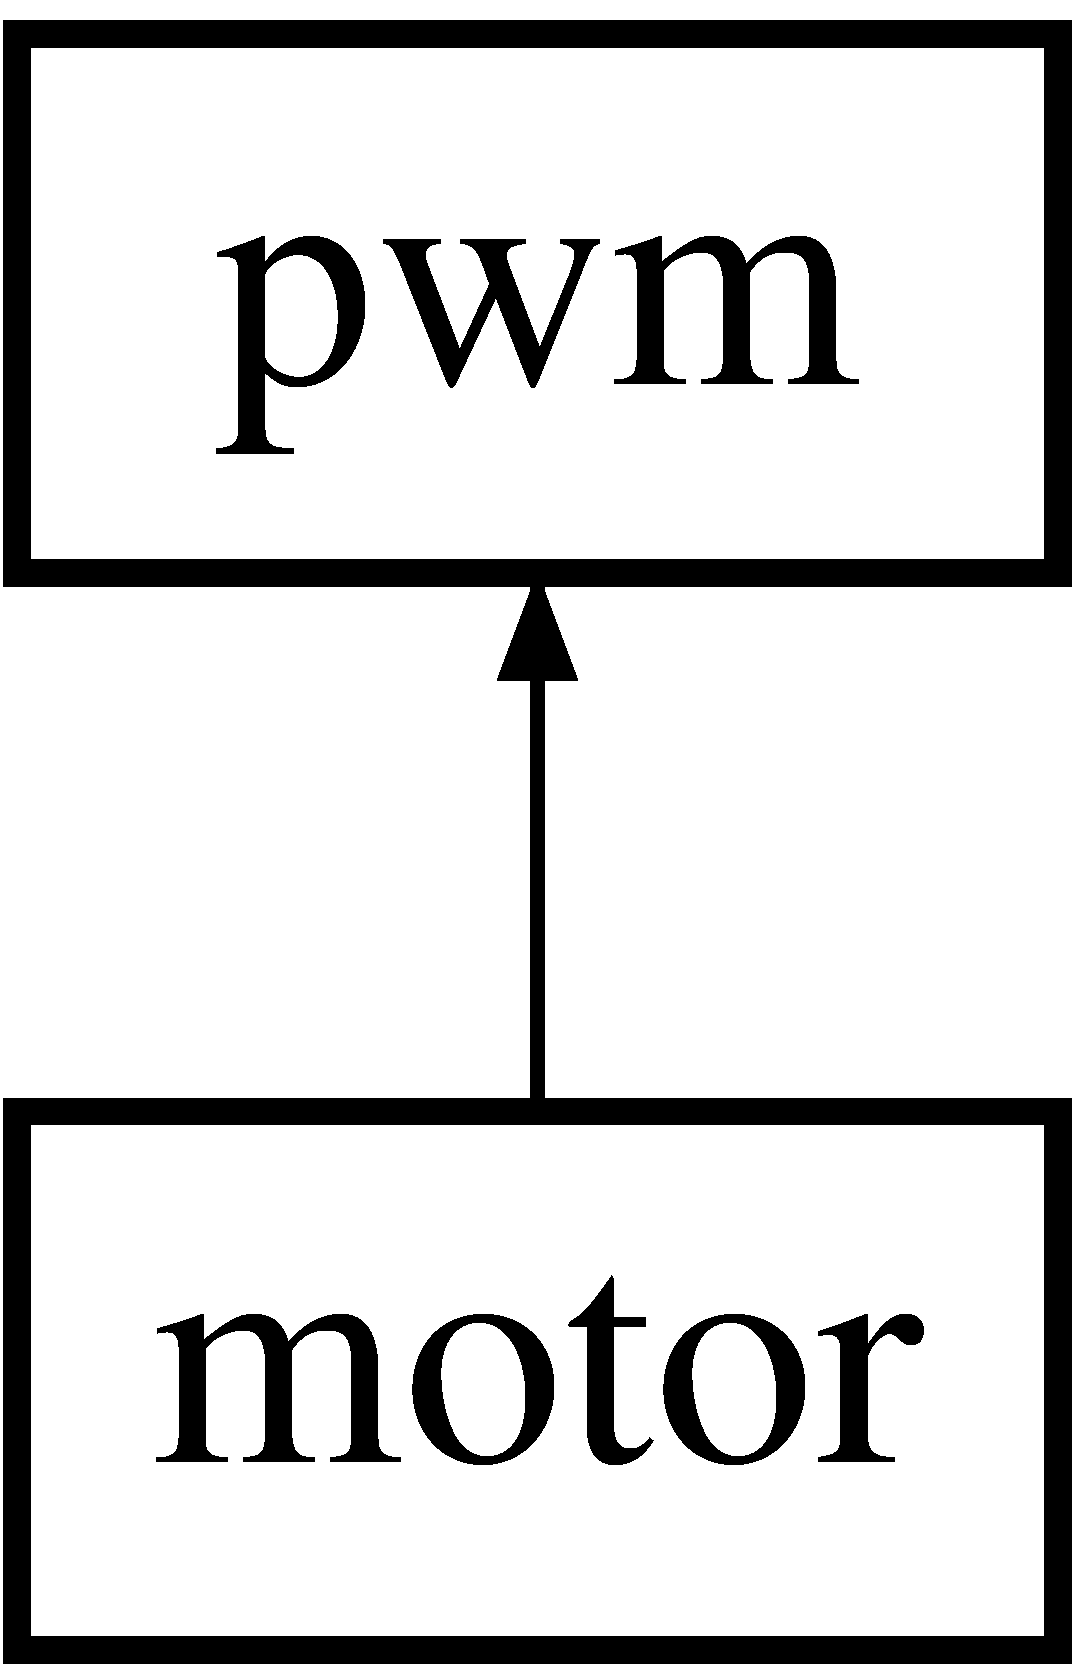
\includegraphics[height=2.000000cm]{classpwm}
\end{center}
\end{figure}
\subsection*{Public Member Functions}
\begin{DoxyCompactItemize}
\item 
\hyperlink{classpwm_a6350bd3cbcdf3a1cf47bd830f41cca59}{pwm} (hwlib\+::target\+::pin\+\_\+out \&pwmpin)
\begin{DoxyCompactList}\small\item\em default constructor \end{DoxyCompactList}\item 
virtual void \hyperlink{classpwm_a028c75f27191dbdbeda2a00ebc27a1eb}{pulse} (int width)
\begin{DoxyCompactList}\small\item\em function for the pwm pulse \end{DoxyCompactList}\end{DoxyCompactItemize}


\subsection{Detailed Description}
class for pwm signal 

this class is for pwm signals 

\subsection{Constructor \& Destructor Documentation}
\index{pwm@{pwm}!pwm@{pwm}}
\index{pwm@{pwm}!pwm@{pwm}}
\subsubsection[{\texorpdfstring{pwm(hwlib\+::target\+::pin\+\_\+out \&pwmpin)}{pwm(hwlib::target::pin_out &pwmpin)}}]{\setlength{\rightskip}{0pt plus 5cm}pwm\+::pwm (
\begin{DoxyParamCaption}
\item[{hwlib\+::target\+::pin\+\_\+out \&}]{pwmpin}
\end{DoxyParamCaption}
)}\hypertarget{classpwm_a6350bd3cbcdf3a1cf47bd830f41cca59}{}\label{classpwm_a6350bd3cbcdf3a1cf47bd830f41cca59}


default constructor 

the cosnstructor sets an pin\+\_\+out for the pwm signal used in this class for this the reference to pin\+\_\+out 

\subsection{Member Function Documentation}
\index{pwm@{pwm}!pulse@{pulse}}
\index{pulse@{pulse}!pwm@{pwm}}
\subsubsection[{\texorpdfstring{pulse(int width)}{pulse(int width)}}]{\setlength{\rightskip}{0pt plus 5cm}void pwm\+::pulse (
\begin{DoxyParamCaption}
\item[{int}]{width}
\end{DoxyParamCaption}
)\hspace{0.3cm}{\ttfamily [virtual]}}\hypertarget{classpwm_a028c75f27191dbdbeda2a00ebc27a1eb}{}\label{classpwm_a028c75f27191dbdbeda2a00ebc27a1eb}


function for the pwm pulse 

this function is for sending the pwm signal. 

The documentation for this class was generated from the following files\+:\begin{DoxyCompactItemize}
\item 
pwm.\+hpp\item 
pwm.\+cpp\end{DoxyCompactItemize}

\hypertarget{class_p_w_m__signal}{}\section{P\+W\+M\+\_\+signal Class Reference}
\label{class_p_w_m__signal}\index{P\+W\+M\+\_\+signal@{P\+W\+M\+\_\+signal}}


Basic P\+WM signal.  




{\ttfamily \#include $<$P\+W\+M\+\_\+signal.\+hpp$>$}

Inheritance diagram for P\+W\+M\+\_\+signal\+:\begin{figure}[H]
\begin{center}
\leavevmode
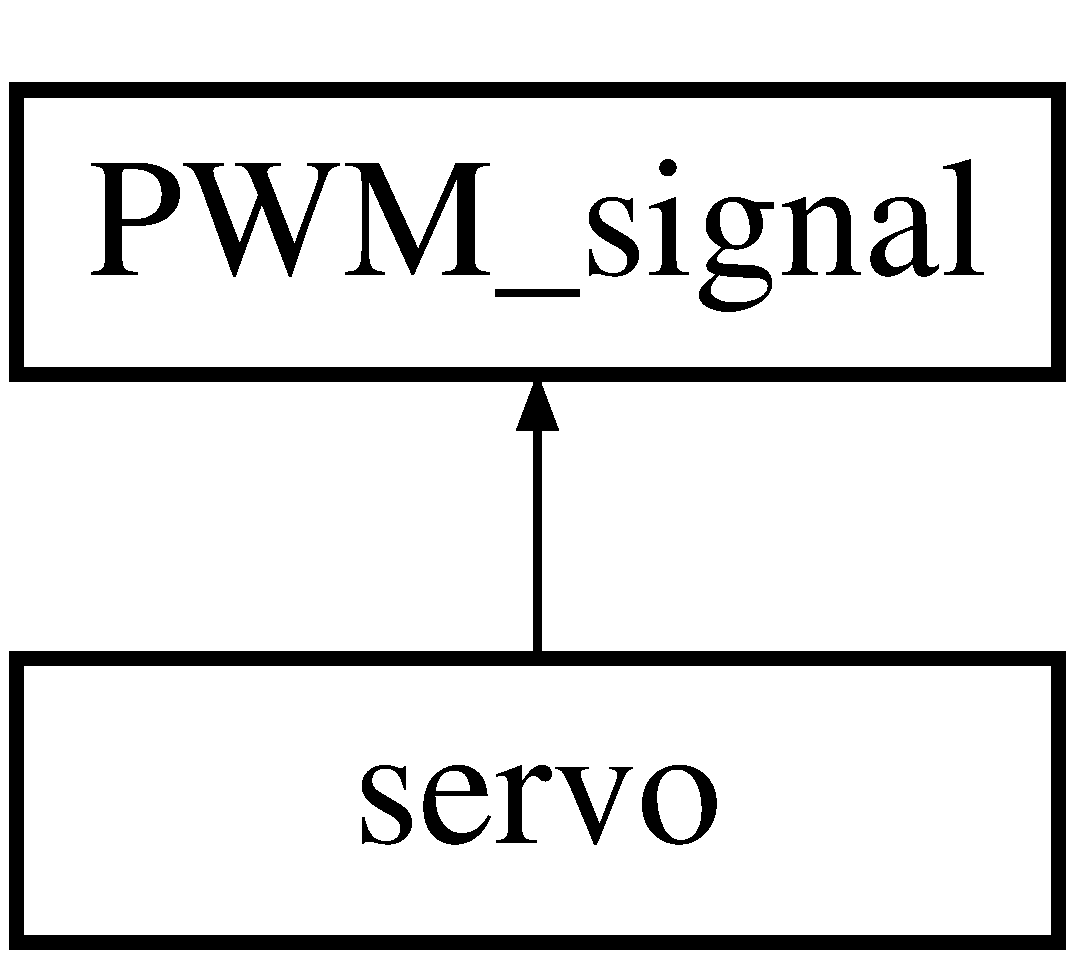
\includegraphics[height=2.000000cm]{class_p_w_m__signal}
\end{center}
\end{figure}
\subsection*{Public Member Functions}
\begin{DoxyCompactItemize}
\item 
\hyperlink{class_p_w_m__signal_ad64aad0e6fe9cf246715bc9cf0f78247}{P\+W\+M\+\_\+signal} (hwlib\+::target\+::pin\+\_\+out \&pwm\+Pin)
\begin{DoxyCompactList}\small\item\em Default constructor. \end{DoxyCompactList}\item 
virtual void \hyperlink{class_p_w_m__signal_a82a9e4648b24a15992b59918e640157c}{P\+W\+M\+\_\+pulse} (int pulse\+Width)
\begin{DoxyCompactList}\small\item\em One pulse. \end{DoxyCompactList}\end{DoxyCompactItemize}


\subsection{Detailed Description}
Basic P\+WM signal. 

This class is for creating a basic P\+WN signal object and then call seperate pules with a certain pulsewidth. 

\subsection{Constructor \& Destructor Documentation}
\index{P\+W\+M\+\_\+signal@{P\+W\+M\+\_\+signal}!P\+W\+M\+\_\+signal@{P\+W\+M\+\_\+signal}}
\index{P\+W\+M\+\_\+signal@{P\+W\+M\+\_\+signal}!P\+W\+M\+\_\+signal@{P\+W\+M\+\_\+signal}}
\subsubsection[{\texorpdfstring{P\+W\+M\+\_\+signal(hwlib\+::target\+::pin\+\_\+out \&pwm\+Pin)}{PWM_signal(hwlib::target::pin_out &pwmPin)}}]{\setlength{\rightskip}{0pt plus 5cm}P\+W\+M\+\_\+signal\+::\+P\+W\+M\+\_\+signal (
\begin{DoxyParamCaption}
\item[{hwlib\+::target\+::pin\+\_\+out \&}]{pwm\+Pin}
\end{DoxyParamCaption}
)}\hypertarget{class_p_w_m__signal_ad64aad0e6fe9cf246715bc9cf0f78247}{}\label{class_p_w_m__signal_ad64aad0e6fe9cf246715bc9cf0f78247}


Default constructor. 

This constructor sets up a pin to control using pwm. It does this using the pin\+\_\+out class in namespace hwlib. 

\subsection{Member Function Documentation}
\index{P\+W\+M\+\_\+signal@{P\+W\+M\+\_\+signal}!P\+W\+M\+\_\+pulse@{P\+W\+M\+\_\+pulse}}
\index{P\+W\+M\+\_\+pulse@{P\+W\+M\+\_\+pulse}!P\+W\+M\+\_\+signal@{P\+W\+M\+\_\+signal}}
\subsubsection[{\texorpdfstring{P\+W\+M\+\_\+pulse(int pulse\+Width)}{PWM_pulse(int pulseWidth)}}]{\setlength{\rightskip}{0pt plus 5cm}void P\+W\+M\+\_\+signal\+::\+P\+W\+M\+\_\+pulse (
\begin{DoxyParamCaption}
\item[{int}]{pulse\+Width}
\end{DoxyParamCaption}
)\hspace{0.3cm}{\ttfamily [virtual]}}\hypertarget{class_p_w_m__signal_a82a9e4648b24a15992b59918e640157c}{}\label{class_p_w_m__signal_a82a9e4648b24a15992b59918e640157c}


One pulse. 

This function is made to create one P\+WM pulse with a user specified pulsewidth. The wait time between every pulse is about 20 ms. 

The documentation for this class was generated from the following files\+:\begin{DoxyCompactItemize}
\item 
\hyperlink{_p_w_m__signal_8hpp}{P\+W\+M\+\_\+signal.\+hpp}\item 
P\+W\+M\+\_\+signal.\+cpp\end{DoxyCompactItemize}

\hypertarget{classservo}{}\section{servo Class Reference}
\label{classservo}\index{servo@{servo}}


Servo controll class.  




{\ttfamily \#include $<$servo.\+hpp$>$}

Inheritance diagram for servo\+:\begin{figure}[H]
\begin{center}
\leavevmode
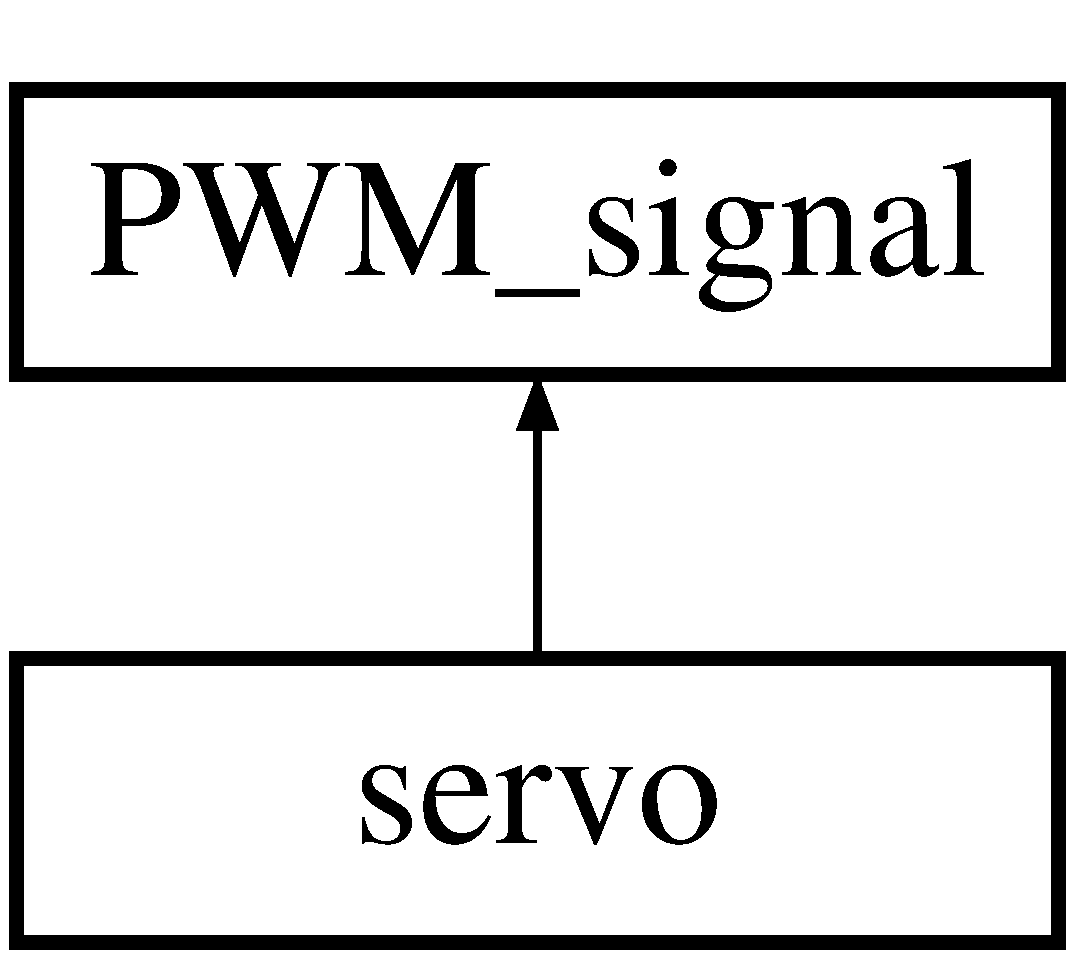
\includegraphics[height=2.000000cm]{classservo}
\end{center}
\end{figure}
\subsection*{Public Member Functions}
\begin{DoxyCompactItemize}
\item 
\hyperlink{classservo_a99c6a39c75cd91b8b2c498cca77d7239}{servo} (hwlib\+::target\+::pin\+\_\+out \&pwm\+Pin)
\begin{DoxyCompactList}\small\item\em Default constructor. \end{DoxyCompactList}\item 
void \hyperlink{classservo_ac0fa39642e5294471844d1fd56e9fec5}{turn\+Degrees} (int degrees)
\begin{DoxyCompactList}\small\item\em Turn the servo to a amount of degrees. \end{DoxyCompactList}\end{DoxyCompactItemize}


\subsection{Detailed Description}
Servo controll class. 

This class is meant to act as a decorator class to the \hyperlink{class_p_w_m__signal}{P\+W\+M\+\_\+signal} class. The idea is that it takes the pulse function and modifies it to send the correct signal for a servo. 

\subsection{Constructor \& Destructor Documentation}
\index{servo@{servo}!servo@{servo}}
\index{servo@{servo}!servo@{servo}}
\subsubsection[{\texorpdfstring{servo(hwlib\+::target\+::pin\+\_\+out \&pwm\+Pin)}{servo(hwlib::target::pin_out &pwmPin)}}]{\setlength{\rightskip}{0pt plus 5cm}servo\+::servo (
\begin{DoxyParamCaption}
\item[{hwlib\+::target\+::pin\+\_\+out \&}]{pwm\+Pin}
\end{DoxyParamCaption}
)}\hypertarget{classservo_a99c6a39c75cd91b8b2c498cca77d7239}{}\label{classservo_a99c6a39c75cd91b8b2c498cca77d7239}


Default constructor. 

This constructor gets a reference to the already existing P\+WM signal taken from the \hyperlink{class_p_w_m__signal}{P\+W\+M\+\_\+signal} class. 

\subsection{Member Function Documentation}
\index{servo@{servo}!turn\+Degrees@{turn\+Degrees}}
\index{turn\+Degrees@{turn\+Degrees}!servo@{servo}}
\subsubsection[{\texorpdfstring{turn\+Degrees(int degrees)}{turnDegrees(int degrees)}}]{\setlength{\rightskip}{0pt plus 5cm}void servo\+::turn\+Degrees (
\begin{DoxyParamCaption}
\item[{int}]{degrees}
\end{DoxyParamCaption}
)}\hypertarget{classservo_ac0fa39642e5294471844d1fd56e9fec5}{}\label{classservo_ac0fa39642e5294471844d1fd56e9fec5}


Turn the servo to a amount of degrees. 

This function get an amount of degrees and then it calculates the wait time. This wait time is beeing given to the pulse function. It also makes sure the servo gets more then one pulse to make sure it has enough time to turn to the set amount of degrees. 

The documentation for this class was generated from the following files\+:\begin{DoxyCompactItemize}
\item 
\hyperlink{servo_8hpp}{servo.\+hpp}\item 
servo.\+cpp\end{DoxyCompactItemize}

\hypertarget{classsound}{}\section{sound Class Reference}
\label{classsound}\index{sound@{sound}}


microphone measure class  




{\ttfamily \#include $<$sound.\+hpp$>$}

Inheritance diagram for sound\+:\begin{figure}[H]
\begin{center}
\leavevmode
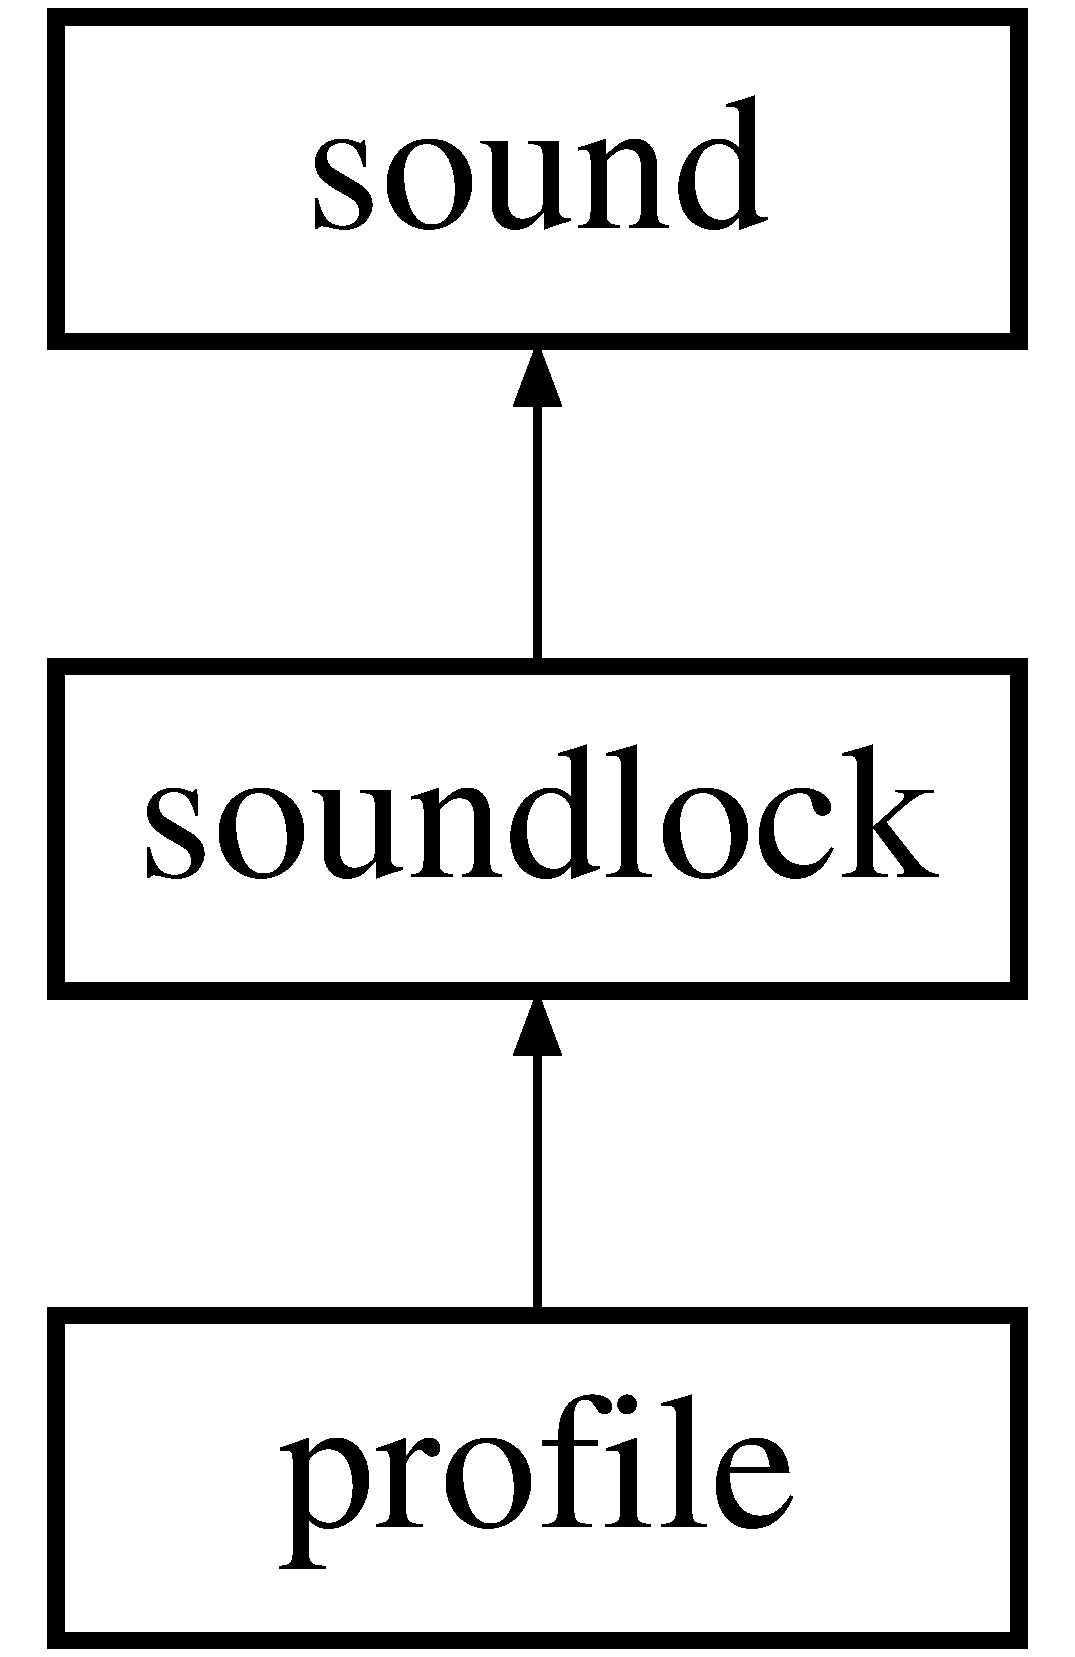
\includegraphics[height=3.000000cm]{classsound}
\end{center}
\end{figure}
\subsection*{Public Member Functions}
\begin{DoxyCompactItemize}
\item 
\hyperlink{classsound_adb8acce21f8278fbf04134748bf8b4d8}{sound} (hwlib\+::target\+::pin\+\_\+adc \&\hyperlink{classsound_a1b4c38e994daa1b3e9006852d3d9242a}{adc})
\begin{DoxyCompactList}\small\item\em default constructor \end{DoxyCompactList}\item 
virtual void \hyperlink{classsound_a40bc8ced8bd7071f1c727a9d4845aade}{measure} ()
\begin{DoxyCompactList}\small\item\em measure function \end{DoxyCompactList}\end{DoxyCompactItemize}
\subsection*{Public Attributes}
\begin{DoxyCompactItemize}
\item 
int \hyperlink{classsound_a5b5e59c09240ddf40827f7c12fafbbad}{array\+\_\+number} = 0\hypertarget{classsound_a5b5e59c09240ddf40827f7c12fafbbad}{}\label{classsound_a5b5e59c09240ddf40827f7c12fafbbad}

\begin{DoxyCompactList}\small\item\em counter that has the length of the measurment\mbox{[}\mbox{]} array after an measurment \end{DoxyCompactList}\end{DoxyCompactItemize}
\subsection*{Protected Attributes}
\begin{DoxyCompactItemize}
\item 
hwlib\+::target\+::pin\+\_\+adc \& \hyperlink{classsound_a1b4c38e994daa1b3e9006852d3d9242a}{adc}\hypertarget{classsound_a1b4c38e994daa1b3e9006852d3d9242a}{}\label{classsound_a1b4c38e994daa1b3e9006852d3d9242a}

\begin{DoxyCompactList}\small\item\em reference to analoge pin used for analoge to digital conversion \end{DoxyCompactList}\item 
int \hyperlink{classsound_a33d9a2a358635cf66a2b08fca23f5a8c}{measurment} \mbox{[}5000\mbox{]}\hypertarget{classsound_a33d9a2a358635cf66a2b08fca23f5a8c}{}\label{classsound_a33d9a2a358635cf66a2b08fca23f5a8c}

\begin{DoxyCompactList}\small\item\em integer array where the measurment are put in \end{DoxyCompactList}\end{DoxyCompactItemize}


\subsection{Detailed Description}
microphone measure class 

This class is for measuring the output of an 3pin ( vcc-\/gnd -\/ a0) microphone 

\subsection{Constructor \& Destructor Documentation}
\index{sound@{sound}!sound@{sound}}
\index{sound@{sound}!sound@{sound}}
\subsubsection[{\texorpdfstring{sound(hwlib\+::target\+::pin\+\_\+adc \&adc)}{sound(hwlib::target::pin_adc &adc)}}]{\setlength{\rightskip}{0pt plus 5cm}sound\+::sound (
\begin{DoxyParamCaption}
\item[{hwlib\+::target\+::pin\+\_\+adc \&}]{adc}
\end{DoxyParamCaption}
)}\hypertarget{classsound_adb8acce21f8278fbf04134748bf8b4d8}{}\label{classsound_adb8acce21f8278fbf04134748bf8b4d8}


default constructor 

this constructor gets and reference of the analoge pin where the microphone is plugged in. 

\subsection{Member Function Documentation}
\index{sound@{sound}!measure@{measure}}
\index{measure@{measure}!sound@{sound}}
\subsubsection[{\texorpdfstring{measure()}{measure()}}]{\setlength{\rightskip}{0pt plus 5cm}void sound\+::measure (
\begin{DoxyParamCaption}
{}
\end{DoxyParamCaption}
)\hspace{0.3cm}{\ttfamily [virtual]}}\hypertarget{classsound_a40bc8ced8bd7071f1c727a9d4845aade}{}\label{classsound_a40bc8ced8bd7071f1c727a9d4845aade}


measure function 

default it will measure 5000 times and place the values into the array measerment\mbox{[}\mbox{]} 

Reimplemented in \hyperlink{classprofile_a5cd64e12649b049cfee501c2e976bd96}{profile}.



The documentation for this class was generated from the following files\+:\begin{DoxyCompactItemize}
\item 
sound.\+hpp\item 
sound.\+cpp\end{DoxyCompactItemize}

\hypertarget{classsoundlock}{}\section{soundlock Class Reference}
\label{classsoundlock}\index{soundlock@{soundlock}}


soundlock class  




{\ttfamily \#include $<$sound\+\_\+lock.\+hpp$>$}

Inheritance diagram for soundlock\+:\begin{figure}[H]
\begin{center}
\leavevmode
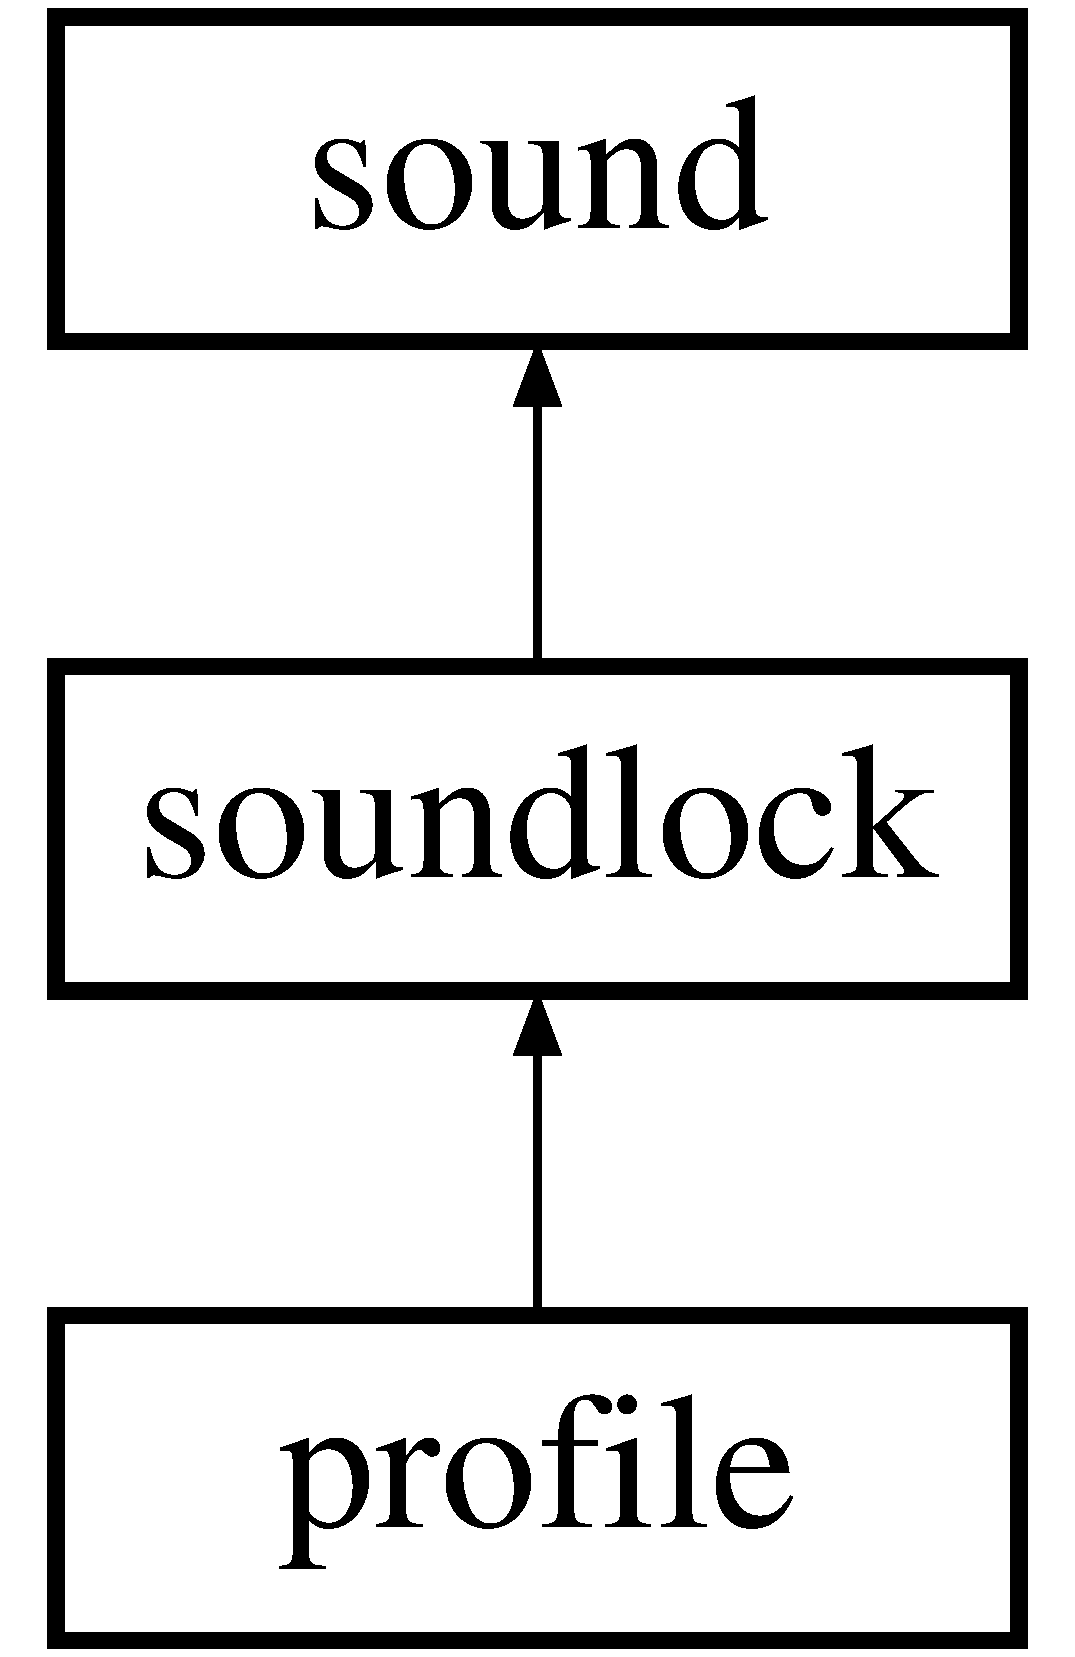
\includegraphics[height=3.000000cm]{classsoundlock}
\end{center}
\end{figure}
\subsection*{Public Member Functions}
\begin{DoxyCompactItemize}
\item 
\hyperlink{classsoundlock_abcac8ac82db4e9cc69c4b0d0ac379a40}{soundlock} (hwlib\+::target\+::pin\+\_\+adc \&\hyperlink{classsound_a1b4c38e994daa1b3e9006852d3d9242a}{adc}, \hyperlink{classlock}{lock} \&\hyperlink{classsoundlock_ade415e22f230dca2d7e7f93d14cec8b6}{l})
\begin{DoxyCompactList}\small\item\em default constructor \end{DoxyCompactList}\item 
virtual void \hyperlink{classsoundlock_ac5e780fa2d0688bee28dbce04dd75a37}{math\+\_\+password} ()=0
\begin{DoxyCompactList}\small\item\em vitual fuction math\+\_\+password \end{DoxyCompactList}\item 
virtual void \hyperlink{classsoundlock_a27ab4e3e5808d7dbc572e865a97e8f9c}{set\+\_\+password} ()=0
\begin{DoxyCompactList}\small\item\em virtual fuction set\+\_\+passsword \end{DoxyCompactList}\item 
virtual void \hyperlink{classsoundlock_abca4638dd9dd78157c2c18165407965e}{compare\+\_\+password} ()=0
\begin{DoxyCompactList}\small\item\em virtual function compare\+\_\+password \end{DoxyCompactList}\end{DoxyCompactItemize}
\subsection*{Protected Attributes}
\begin{DoxyCompactItemize}
\item 
\hyperlink{classpassword}{password} \hyperlink{classsoundlock_a3de94ef881d8470d0217276e0f613cf1}{temp}\hypertarget{classsoundlock_a3de94ef881d8470d0217276e0f613cf1}{}\label{classsoundlock_a3de94ef881d8470d0217276e0f613cf1}

\begin{DoxyCompactList}\small\item\em temparary password for comparing an setting password. \end{DoxyCompactList}\item 
\hyperlink{classlock}{lock} \& \hyperlink{classsoundlock_ade415e22f230dca2d7e7f93d14cec8b6}{l}\hypertarget{classsoundlock_ade415e22f230dca2d7e7f93d14cec8b6}{}\label{classsoundlock_ade415e22f230dca2d7e7f93d14cec8b6}

\begin{DoxyCompactList}\small\item\em reference to an lock that is needed for controlling \end{DoxyCompactList}\end{DoxyCompactItemize}
\subsection*{Additional Inherited Members}


\subsection{Detailed Description}
soundlock class 

decorator class to the sound class for controllling an lock 

\subsection{Constructor \& Destructor Documentation}
\index{soundlock@{soundlock}!soundlock@{soundlock}}
\index{soundlock@{soundlock}!soundlock@{soundlock}}
\subsubsection[{\texorpdfstring{soundlock(hwlib\+::target\+::pin\+\_\+adc \&adc, lock \&l)}{soundlock(hwlib::target::pin_adc &adc, lock &l)}}]{\setlength{\rightskip}{0pt plus 5cm}soundlock\+::soundlock (
\begin{DoxyParamCaption}
\item[{hwlib\+::target\+::pin\+\_\+adc \&}]{adc, }
\item[{{\bf lock} \&}]{l}
\end{DoxyParamCaption}
)}\hypertarget{classsoundlock_abcac8ac82db4e9cc69c4b0d0ac379a40}{}\label{classsoundlock_abcac8ac82db4e9cc69c4b0d0ac379a40}


default constructor 

theconstructor gets an reference to an analog port that is used for the analog to digital conversion . and a reference to an lock that is used to control. 

\subsection{Member Function Documentation}
\index{soundlock@{soundlock}!compare\+\_\+password@{compare\+\_\+password}}
\index{compare\+\_\+password@{compare\+\_\+password}!soundlock@{soundlock}}
\subsubsection[{\texorpdfstring{compare\+\_\+password()=0}{compare_password()=0}}]{\setlength{\rightskip}{0pt plus 5cm}virtual void soundlock\+::compare\+\_\+password (
\begin{DoxyParamCaption}
{}
\end{DoxyParamCaption}
)\hspace{0.3cm}{\ttfamily [pure virtual]}}\hypertarget{classsoundlock_abca4638dd9dd78157c2c18165407965e}{}\label{classsoundlock_abca4638dd9dd78157c2c18165407965e}


virtual function compare\+\_\+password 

default doing nothing can be set for comparing password with input 

Implemented in \hyperlink{classprofile_acefbce03d19dafccbcf55c17b3527a23}{profile}.

\index{soundlock@{soundlock}!math\+\_\+password@{math\+\_\+password}}
\index{math\+\_\+password@{math\+\_\+password}!soundlock@{soundlock}}
\subsubsection[{\texorpdfstring{math\+\_\+password()=0}{math_password()=0}}]{\setlength{\rightskip}{0pt plus 5cm}virtual void soundlock\+::math\+\_\+password (
\begin{DoxyParamCaption}
{}
\end{DoxyParamCaption}
)\hspace{0.3cm}{\ttfamily [pure virtual]}}\hypertarget{classsoundlock_ac5e780fa2d0688bee28dbce04dd75a37}{}\label{classsoundlock_ac5e780fa2d0688bee28dbce04dd75a37}


vitual fuction math\+\_\+password 

default doing nothing can be set for calculating password for lock 

Implemented in \hyperlink{classprofile_a85a7931430f0cc2abc94253548b9cb37}{profile}.

\index{soundlock@{soundlock}!set\+\_\+password@{set\+\_\+password}}
\index{set\+\_\+password@{set\+\_\+password}!soundlock@{soundlock}}
\subsubsection[{\texorpdfstring{set\+\_\+password()=0}{set_password()=0}}]{\setlength{\rightskip}{0pt plus 5cm}virtual void soundlock\+::set\+\_\+password (
\begin{DoxyParamCaption}
{}
\end{DoxyParamCaption}
)\hspace{0.3cm}{\ttfamily [pure virtual]}}\hypertarget{classsoundlock_a27ab4e3e5808d7dbc572e865a97e8f9c}{}\label{classsoundlock_a27ab4e3e5808d7dbc572e865a97e8f9c}


virtual fuction set\+\_\+passsword 

default doing nothing can be set for setting te password for the lock 

Implemented in \hyperlink{classprofile_aa46b5ea874a915a76a54c4ce7fa9701c}{profile}.



The documentation for this class was generated from the following files\+:\begin{DoxyCompactItemize}
\item 
sound\+\_\+lock.\+hpp\item 
sound\+\_\+lock.\+cpp\end{DoxyCompactItemize}

\chapter{File Documentation}
\hypertarget{_p_w_m__signal_8hpp}{}\section{P\+W\+M\+\_\+signal.\+hpp File Reference}
\label{_p_w_m__signal_8hpp}\index{P\+W\+M\+\_\+signal.\+hpp@{P\+W\+M\+\_\+signal.\+hpp}}
{\ttfamily \#include \char`\"{}hwlib.\+hpp\char`\"{}}\\*
\subsection*{Classes}
\begin{DoxyCompactItemize}
\item 
class \hyperlink{class_p_w_m__signal}{P\+W\+M\+\_\+signal}
\begin{DoxyCompactList}\small\item\em Basic P\+WM signal. \end{DoxyCompactList}\end{DoxyCompactItemize}

\hypertarget{servo_8hpp}{}\section{servo.\+hpp File Reference}
\label{servo_8hpp}\index{servo.\+hpp@{servo.\+hpp}}
{\ttfamily \#include \char`\"{}P\+W\+M\+\_\+signal.\+hpp\char`\"{}}\\*
{\ttfamily \#include \char`\"{}hwlib.\+hpp\char`\"{}}\\*
\subsection*{Classes}
\begin{DoxyCompactItemize}
\item 
class \hyperlink{classservo}{servo}
\begin{DoxyCompactList}\small\item\em Servo controll class. \end{DoxyCompactList}\end{DoxyCompactItemize}
\subsection*{Macros}
\begin{DoxyCompactItemize}
\item 
\#define {\bfseries M\+A\+X\+\_\+\+D\+E\+G\+R\+E\+ES}~360\hypertarget{servo_8hpp_a4ba510f21f53f375dd98267c4a644281}{}\label{servo_8hpp_a4ba510f21f53f375dd98267c4a644281}

\item 
\#define {\bfseries M\+I\+N\+\_\+\+D\+E\+G\+R\+E\+ES}~0\hypertarget{servo_8hpp_a0433cf7215e086e910d2fc9f84c25e79}{}\label{servo_8hpp_a0433cf7215e086e910d2fc9f84c25e79}

\end{DoxyCompactItemize}

%--- End generated contents ---

% Index
\backmatter
\newpage
\phantomsection
\clearemptydoublepage
\addcontentsline{toc}{chapter}{Index}
\printindex

\end{document}
